\section{Introduction}\label{introduction}

Scalable photonic computing marks a pivotal shift in high-performance system architecture, driven by the escalating energy demands of artificial intelligence and the physical limits of electronic interconnects. As data-centric workloads increasingly dominate computational landscapes, the traditional reliance on charge-based transport faces fundamental bottlenecks in bandwidth density and energy efficiency. Integrated photonics offers a compelling alternative, leveraging the inherent parallelism of light to perform linear algebra operations with potentially orders-of-magnitude lower energy consumption per operation. However, the transition from isolated device demonstrations to wafer-scale, programmable systems is not merely a matter of scaling component counts. It requires navigating a complex landscape of material trade-offs, architectural constraints, and systemic physical limitations that define the current state of ODNN research.

Material platform selection serves as the cornerstone of scalable photonic systems, imposing fundamental constraints on performance. Silicon photonics remains the dominant candidate for dense integration due to its compatibility with complementary metal-oxide-semiconductor (CMOS) fabrication ecosystems, yet it suffers from weak electro-optic effects and nonlinear losses at high powers. Conversely, thin-film lithium niobate (TFLN) offers superior modulation efficiency and low loss, as evidenced by recent advances in sunken dual-layer electrode designs achieving half-wave voltage-length products below 1.6 V \(\cdot\) cm \citep{doi_10_3390_photonics12111129_03f4b6cd}. However, TFLN currently lacks the mature foundry infrastructure required for large-scale logic integration. This dichotomy suggests that no single material platform currently satisfies all requirements for scale, speed, and energy efficiency simultaneously, necessitating hybrid integration strategies that combine disparate materials on a single substrate.

Drawing on these physical foundations, programmable photonic circuit architectures have emerged as the primary mechanism for implementing reconfigurable linear transformations. The Mach-Zehnder interferometer (MZI) mesh serves as the canonical building block, capable of realizing universal unitary transformations essential for photonic neural networks and quantum information processing. Recent experimental demonstrations on general-purpose silicon photonic platforms have validated the programming of hexagonal waveguide meshes, achieving fidelities exceeding 98\% for small-scale unitary matrices \citep{doi_10_1063_5_0235712_fb28986d}. These architectures enable the construction of photonic matrix multiplication engines, which exploit optical interference to perform parallel dot-product operations. While such engines demonstrate transformative advantages in energy-per-MAC for low-precision inference, their applicability is structurally limited by the absence of native nonlinearity in passive media. Consequently, photonic accelerators function most effectively as specialized co-processors for static or slowly varying linear transformations, rather than as universal replacements for electronic graphics processing units.

Despite these promising capabilities, the scalability of practical photonic computing systems is constrained by compounding physical effects that degrade signal fidelity in dense arrays. The primary tension in ODNN research arises from the conflict between the theoretical efficiency of optical computing and the practical realities of thermal crosstalk, cascaded insertion loss, and fabrication-induced variations. In dense programmable meshes, thermo-optic phase shifters introduce significant thermal crosstalk, perturbing neighboring elements and necessitating complex calibration protocols that erode energy benefits \citep{doi_10_1109_access_2020_3013116_8fec1fb2}. Furthermore, the lack of efficient all-optical activation functions forces reliance on hybrid optoelectronic interfaces for nonlinear operations, introducing latency and power overheads that can negate theoretical gains. This reality is particularly acute for dynamic training workloads requiring frequent weight updates and gradient computations, where the rigidity of optical hardware presents a fundamental mismatch with algorithmic requirements. Recent analyses of photonic transformer accelerators highlight these challenges, noting that while convolutional workloads map well to static photonic cores, attention-based mechanisms demand dynamic reconfiguration that current hardware struggles to support efficiently \citep{doi_10_1109_hpca57654_2024_00059_f488ee7a}.

This review synthesizes the emerging paradigm of electronic-photonic co-design, which treats hardware geometry, control electronics, and algorithmic structure as a unified optimization problem to address these systemic bottlenecks. Rather than optimizing devices in isolation, co-design methodologies leverage physics-informed machine learning and inverse design tools to automate the mapping of abstract computational objectives to manufacturable device geometries. Intelligent design automation frameworks, such as those combining fabrication-aware inverse design with routing-informed placement, are beginning to bridge the gap between theoretical performance and practical realizability \citep{doi_10_1117_12_3066105_d6297c38}. The resulting design extends to system-level applications, where optical interconnect fabrics offer an immediately deployable solution for bandwidth bottlenecks. Architectures like OptoLink demonstrate the potential of photonic interconnects to alleviate memory bandwidth constraints in specialized accelerators, achieving terabit-scale throughput with significantly reduced latency compared to electrical networks \citep{doi_10_1145_3806395_315ab915}.

This review follows a logical progression from physical constraints to system-level solutions. Section S01 establishes the material physics governing device performance, followed by Section S02 and Section S03, which detail programmable architectures and matrix multiplication engines, respectively. Section S06 critically examines the scalability bottlenecks of loss, crosstalk, and control complexity that define the problem space. Section S07 then presents electronic-photonic co-design methodologies as the strategic response to these challenges. Finally, Sections S04 and S05 evaluate system-level applications in AI acceleration and optical interconnects, culminating in Section S08, which synthesizes the current trajectory of ODNN research and identifies critical gaps in benchmarking and standardization. Through this structured analysis, we argue that the future of scalable photonic computing lies not in isolated breakthroughs in device metrics, but in the synergistic integration of heterogeneous platforms, intelligent design algorithms, and rigorous system-level validation.

\section{Device Physics and Material Platforms for Scalable Photonic Computing Integration}\label{device-physics-and-material-platforms-for-scalable-photonic-computing-integration}

Scalable photonic computing design spaces are fundamentally shaped by the material dichotomy between silicon photonics and thin-film lithium niobate (TFLN). Silicon photonics provides a high-density, CMOS-compatible platform essential for dense integration, yet it is intrinsically limited by the absence of a linear electro-optic effect and significant two-photon absorption losses at high optical intensities. \citep{doi_10_3390_photonics11040375_bd102ef0} \citep{doi_10_3390_photonics12010005_5e399e5f} In contrast, TFLN leverages the strong Pockels electro-optic modulation and low propagation loss characteristic of ferroelectric crystals, making it suitable for high-speed, energy-efficient operations, though it currently faces challenges in achieving the integration density of silicon. \citep{doi_10_3390_photonics12111129_03f4b6cd} \citep{doi_10_3390_mi17060751_d3932b5d} Bridging these extremes, silicon nitride exhibits a nonlinear susceptibility of approximately 2.5 \(\times\) 10\(^{-19}\) m\(^{2}\)/W at 1.55 \(\mu\) m, enabling efficient four-wave mixing processes suitable for applications such as Kerr microcomb generation. Furthermore, silicon nitride benefits from ultra-low propagation loss in the visible and near-infrared spectral windows, although its weak electro-optic response similarly necessitates auxiliary modulation schemes. This trade-off creates a critical bottleneck: while silicon benefits from mature fabrication ecosystems, its reliance on thermo-optic phase shifters introduces inevitable thermal crosstalk that can lead to erroneous signal routing and restricts working capabilities in dense networks. Consequently, the choice of material platform constrains the achievable scale, speed, and energy efficiency of integrated circuits, necessitating hybrid integration strategies to balance the conflicting demands of fabrication maturity, loss, and speed. \citep{doi_10_48550_arxiv_2209_10098_b3bedb78} \citep{doi_10_1126_science_abj4396_40f36a09} \citep{doi_10_1149_ma2026_01311465mtgabs_643e381a} \citep{doi_10_1109_access_2020_3013116_8fec1fb2}

The implementation of matrix-vector multiplication (MVM)---the core operation in optical neural networks---relies on three dominant architectural primitives established by prior material constraints: free-space diffraction systems, Mach-Zehnder interferometer (MZI) arrays, and micro-ring resonator (MRR) networks. \citep{doi_10_1088_1402_4896_ae8345_3b948559} Free-space systems utilize diffraction layers to perform computations with high throughput but are inherently bulky, difficult to integrate on-chip, and challenging to tune for scalable applications. In contrast, integrated solutions based on MZI arrays and MRRs offer compact structures suitable for chip-scale photonic computing, yet they introduce distinct physical vulnerabilities. These integrated approaches require extremely precise phase control and complex feedback circuits to function, often suffering from high power consumption, poor stability, and scalability limits imposed by waveguide cross-talk and propagation loss. A third pathway, Diffractive Optical Neural Networks (DONNs), has emerged to bridge these gaps; while initially developed in free-space, DONNs are now implemented on-chip to enhance compatibility with photonic circuits, offering passive low-power operation and ultrahigh throughput. However, like their integrated counterparts, these on-chip diffractive architectures must navigate complex optical constraints to achieve reconfigurability. Ultimately, the choice among these architectures represents a critical trade-off between the scalability and programmability of integrated devices versus the bulk and tuning difficulties of free-space systems, setting the stage for the thermal and fabrication stability challenges that limit their large-scale deployment. \citep{doi_10_1088_1402_4896_ae8345_3b948559} \citep{doi_10_1002_nap2_70098_8d5f2f8a}

Figure \ref{fig:visual_01} illustrates key material properties (electro-optic coefficient, propagation loss, nonlinear effects, CMOS compatibility, modulation speed, fabrication maturity) across silicon photonics, thin-film lithium niobate, indium\ldots{}

\begin{figure}
\centering

\includegraphics[width=0.9\linewidth,height=\textheight,keepaspectratio,alt={Photonic Material Platform Trade-off Landscape. No single platform dominates all metrics, requiring selection based on specific computing workload priorities like speed versus integration density. AI-assisted explanatory diagram; not empirical evidence.}]{figures/01_FIG-GEN-001.png}
\caption{Photonic Material Platform Trade-off Landscape. No single platform dominates all metrics, requiring selection based on specific computing workload priorities like speed versus integration density. AI-assisted explanatory diagram; not empirical evidence.}\label{fig:visual_01}
\end{figure}

Physical noise sources inherent to the material platform fundamentally degrade the fidelity of architectural primitives like MZI arrays when scaling complex matrix operations. In silicon photonic integrated circuits, thermal crosstalk arises from the inevitable thermal conductance of chip materials, where heating intended for one component creates undesired phase shifts in adjacent waveguides. \citep{doi_10_1109_access_2020_3013116_8fec1fb2} This phenomenon acts as a dominant error mechanism in dense arrays of thermo-optic phase shifters and attenuators, potentially leading to erroneous signal routing and reduced output power. Although strategies such as three-dimensional trenches or doped silicon heaters have been proposed to localize heating effects, comprehensive analysis remains limited by heat dissipation through the silicon substrate. Compounding these thermal issues are fabrication variations, specifically finite precision in waveguide width and thickness, which introduce fundamental phase noise that corrupts matrix-vector multiplication in coherent nanophotonic neural networks. \citep{doi_10_1109_tnano_2022_3223915_d4da3e6b} The sensitivity of these devices to such variations scales directly with nominal dimensions, though optimized ridge waveguide designs have shown resilience against expected levels of non-uniformity. Furthermore, while photonic resonators offer advantageous nonlinear behavior for implementing activation functions, they remain acutely vulnerable to environmental factors like temperature fluctuations and mechanical vibrations, necessitating sophisticated control mechanisms to maintain stability. These intertwined constraints of thermal management, fabrication tolerance, and environmental sensitivity illustrate that scaling photonic computing is a design challenge and a battle against intrinsic physical limitations. \citep{doi_10_1109_access_2020_3013116_8fec1fb2} \citep{doi_10_1109_tnano_2022_3223915_d4da3e6b} \citep{doi_10_3390_nano14080697_c372a140}

Heterogeneous back-end-of-line (BEOL) integration has emerged as a primary unifying strategy to address the conflicting demands of high-speed modulation and dense CMOS-compatible routing identified in previous scaling barriers. This method involves bonding thin-film lithium niobate (TFLN), a material defined by its strong Pockels electro-optic effect, directly onto active silicon photonics platforms after the standard silicon circuitry is fabricated. \citep{s2_9b444e84d20ae6e3d62d2d4df30268b5a53baad2_40af2cc9} By combining these layers, the platform leverages the intrinsically low loss and superior modulation efficiency of TFLN while retaining the mature, highly integrated design kits of silicon photonics for dense routing and detection. Recent demonstrations confirm that the optical architecture overcomes key die-to-wafer bonding challenges to integrate high-performance modulators with germanium photodetectors on a single chip, creating a clear path toward scalable transceivers for optical networks-on-chip. Complementing this vertical stacking, on-chip dielectric metasurfaces offer a unique scheme to control the degrees of freedom of the light field within a compact footprint. Compatible with standard CMOS fabrication, these metasurfaces function as arbitrary wavefront shapers capable of performing analog mathematical operations like convolution, positioning them as promising candidates for broadband, low-loss photonic computing accelerators. Demonstrating this capability, a monolithic metasurface spatial differentiator was developed based on asymmetric photonic spin-orbit interactions to perform edge detection. The device operates using the polarization degree and functions within a broadband range, offering a more compact alternative to bulky optical analog systems. \citep{doi_10_1515_nanoph_2020_0366_58f1aa1d} While reconfigurability in metasurface devices remains an area of active development, the convergence of heterogeneous BEOL integration and metasurface functionality illustrates a critical direction for overcoming the material dichotomy: merging the best physical properties of disparate platforms to enable wafer-scale systems, though full realization of these hybrid strategies requires further methodological development. \citep{s2_9b444e84d20ae6e3d62d2d4df30268b5a53baad2_40af2cc9} \citep{doi_10_1515_nanoph_2022_0294_1bd118d5}

Inverse design methodologies address the remaining geometric rigidity inherent in traditional device layouts by determining optimal geometries directly from desired optical responses, thereby complementing hybrid integration strategies that resolve material conflicts. \citep{doi_10_1364_oe_524318_cf5f0d79} \citep{doi_10_1364_ol_453299_4bc70b17} Unlike conventional intuition-driven design, this method employs optimization algorithms and deep learning to navigate complex parameter spaces, generating structures that meet specific performance targets while mitigating fabrication tolerance constraints by creating robust modes less sensitive to minor geometric variations. The mechanism typically relies on replacing computationally intensive electromagnetic simulations, such as Monte Carlo or finite-difference time-domain solvers, with deep learning surrogates that enable efficient gradient-based optimization of complex geometries like scintillators and power splitters. \citep{doi_10_1109_jmmct_2026_3695747_9d633c4d} \citep{doi_10_17725_j_rensit_2026_18_163_741010b8} However, this flexibility is not absolute; the accessible design space remains strictly constrained by fabrication tolerances, specifically minimum feature sizes and length scale limits. For instance, approaches using coarse grids to enforce these constraints can confine the search to a tiny subset of possible outcomes, resulting in optimal structures with significantly lower efficiency compared to those found within a broader, physics-informed search space. Furthermore, while artificial intelligence can generate optimized designs rapidly after training, the process demands an extensive number of initial simulations, creating a significant one-time computational cost that scales with structural complexity. Ultimately, the performance of these AI-generated devices cannot exceed the capabilities present within their training datasets, indicating that inverse design serves as a powerful tool for navigating material-platform trade-offs but requires careful management of computational resources and physical boundaries to realize scalable photonic computing. \citep{doi_10_1515_nanoph_2024_0536_4b6631ba} \citep{doi_10_1515_nanoph_2023_0852_cb27a26f} \citep{doi_10_1109_cleo_europe_eqec65582_2025_11110329_26a41a7d}

Inverse design algorithms effectively navigate complex geometric spaces, yet their reliance on traditional numerical solvers creates a computational bottleneck for wafer-scale circuits. Deep learning surrogates address this by replacing expensive finite-difference frequency domain simulations with rapid neural approximations. Specifically, neural operators have emerged as a powerful framework that learns mappings between function spaces, such as taking material coefficients or boundary conditions as inputs to directly return solution fields, rather than regressing fixed-dimensional vectors. \citep{doi_10_48550_arxiv_2303_10506_0452bde4} Once trained, these models evaluate new designs at negligible cost while remaining differentiable, a property essential for gradient-based optimization. Practical implementations demonstrate this efficiency; for instance, deep neural networks trained on thousands of simulation data points can predict the spectral response of integrated photonic power splitters in a fraction of a second, enabling rapid inverse design where user-specified optical responses map immediately to device topologies. Surrogate scattering-matrix inverse design enables the scalable creation of photonic neural networks by leveraging learned models to bypass traditional simulation bottlenecks. \citep{s2_753a5d83a96e0194da93bcb6f20fa0bd356e37fa_c11e3796} Furthermore, physics-informed approaches and adjoint-based methods leverage these capabilities to tackle PDE-constrained optimal control problems, offering a pathway to overcome the scaling limits inherent in conventional simulation workflows. By decoupling design iteration from heavy numerical solving, these surrogate models provide the computational speed necessary to realize the dense, high-performance architectures demanded by scalable photonic computing. \citep{doi_10_48550_arxiv_2601_00199_c689b34d} \citep{doi_10_1038_s41598_018_37952_2_076b64f9} \citep{doi_10_48550_arxiv_2606_12337_68b62bfa}

The utility of neural surrogates in accelerating candidate design generation is fundamentally bounded by generalization limits and the rugged topology of photonic objective landscapes. Deep learning frameworks often fail to extrapolate beyond the specific geometries and spectra present in their training datasets, restricting their ability to propose novel structures without additional refinement. To overcome this, hybrid algorithms have emerged that pair neural networks for global search with conventional optimization methods, such as adjoint-based techniques, to perform local refinement. Furthermore, the physical nature of photonic devices introduces severe mathematical challenges; for instance, in Distributed Bragg Reflectors, cyclic interference between waves creates highly oscillatory objective functions riddled with local minima that confound standard gradient-based optimizers like Adam or L-BFGS. Although artificial intelligence significantly speeds up the design cycle, the reliability of these outputs remains contingent on the fidelity of underlying physics models and the computational cost of generating sufficient training data through electromagnetic simulations. Consequently, achieving robust, wafer-scale integration requires moving beyond pure data-driven approaches to methods that can navigate these irregular loss landscapes and generalize across diverse material platforms. \citep{doi_10_1021_acsphotonics_2c00968_06a2e96b} \citep{doi_10_48550_arxiv_2602_18148_e9c0a72b} \citep{doi_10_1515_nanoph_2024_0536_4b6631ba}

ODNN research is converging on a synthesis of hybrid integration and AI-driven inverse design to overcome the material and fabrication bottlenecks identified in previous sections. Physics-informed machine learning emerges as a critical enabler for managing the complexity of wafer-scale photonic circuits, allowing for the optimization of device performance despite high-dimensional design spaces and strict fabrication limitations. By embedding governing physical laws directly into the learning process, these methods reduce data dependency while hybrid frameworks synergistically combine deep learning with classical optimization techniques like adjoint methods to ensure robust convergence. For instance, cost-efficient deep learning surrogates have successfully optimized meta-atom geometries for specific diffraction targets, navigating constraints such as fixed material heights and lithography resolution limits that would stall traditional iterative approaches. This computational leverage complements the physical advantages of photonic integrated circuits (PICs), which offer superior energy efficiency and scalability compared to conventional electronic systems, particularly for solving combinatorial optimization problems like the traveling salesman problem through massive parallelism. Ultimately, the path to scalable photonic computing relies not on a single breakthrough but on this dual strategy: using intelligent algorithms to maximize the potential of heterogeneous material platforms, thereby transforming physical constraints into manageable design parameters. \citep{doi_10_1109_sbfotoniopc62248_2024_10813471_692f0088} \citep{doi_10_1021_acsami_5c03196_32a62b73} \citep{doi_10_3390_nano14080697_c372a140}

\section{Programmable Photonic Circuit Architectures and Reconfigurable Mesh Topologies for Photonic Computing}\label{programmable-photonic-circuit-architectures-and-reconfigurable-mesh-topologies-for-photonic-computing}

Programmable photonic computing relies on the Mach-Zehnder interferometer (MZI) mesh as its fundamental building block, enabling universal unitary transformations through precise phase-controlled interference. \citep{doi_10_48550_arxiv_2407_03235_fe345c4b} \citep{doi_10_1063_5_0235712_fb28986d} In these coherent arrays, light is split, subjected to tunable phase shifts, and recombined to execute linear algebra operations directly at the speed of light. This architecture has emerged as a mainstream solution for optical matrix-vector multiplication on integrated chips, standing alongside free-space diffraction systems and micro-ring resonator networks as a primary approach to overcoming the bandwidth and energy efficiency limits of electronic accelerators in the post-Moore's law era. By leveraging silicon photonics, MZI-based systems promise to reduce the complexity of matrix operations significantly while offering negligible latency for inferencing tasks. However, despite their potential as a promising alternative to traditional electronics, these integrated solutions face substantial bottlenecks when scaling toward high-density integration; they require extremely precise phase control and complex feedback circuits, and remain vulnerable to fabrication-process variations that can cause catastrophic accuracy loss without individual calibration. This tension between the theoretical capability for universal transformation and the practical challenges of stability and control defines the current landscape of programmable photonic architectures. \citep{doi_10_1109_tnano_2022_3223915_d4da3e6b} \citep{doi_10_1088_1402_4896_ae8345_3b948559}

Diffractive optical neural networks (DONNs) provide a static, passive alternative to programmable Mach-Zehnder interferometer meshes, which offer universal unitary transformations through active tuning. DONNs implement linear transformations via physical diffraction layers and, unlike the reconfigurable but power-hungry interferometric arrays, leverage their scalability in neuron number and ultrahigh throughput to achieve low-power operation for specific machine learning tasks, evolving from foundational free-space implementations to integrated on-chip configurations compatible with photonic circuits. A representative advancement in this domain is the photonic crystal diffractive optical neural network (PhC-DONN), which utilizes two-dimensional photonic crystals to enable multi-wavelength parallel processing for on-chip optical classification. By establishing a wavelength-diffraction joint modulation model, the PhC-DONN overcomes the inherent limitations of traditional single-wavelength diffractive networks, demonstrating exceptional performance in image and video classification while offering a pathway toward high-efficiency optical artificial intelligence processors. Although these static architectures lack the dynamic reconfigurability of MZI meshes, their ability to perform fixed linear operations with minimal energy consumption highlights a critical trade-off in photonic computing design, setting the stage for inverse design techniques that can further optimize such non-standard topologies beyond human intuition. \citep{doi_10_1002_nap2_70098_8d5f2f8a} \citep{doi_10_1515_nanoph_2025_0168_86a0f7aa}

Moving beyond the fixed transformations of static diffractive networks and the regular geometries of standard MZI arrays, nanophotonic inverse design represents a paradigm shift that overcomes the inherent limitations of intuition-based manual engineering. \citep{doi_10_1088_1361_6633_ae7f9a_e05f9b1d} \citep{doi_10_1109_icufn61752_2024_10625552_985a60f2} This computational approach determines device geometry directly from desired optical responses, enabling the implementation of non-intuitive circuit topologies that traditional heuristic methods cannot conceive. Unlike conventional trial-and-error modeling which relies on incremental advancements through repeated simulation cycles, inverse design algorithms navigate the full parameter space to minimize cost functions, often revealing complex structures with optimal performance that defy human geometric expectations. The integration of artificial intelligence and deep learning further accelerates this process; while generating the initial training datasets requires significant computational effort, trained neural networks can subsequently solve design requests almost instantaneously. These data-driven models capture complex physical relationships between material properties and optical responses, allowing for the simultaneous optimization of higher-level figures of merit and the rapid convergence of design parameters. By fusing optimization schemes with deep learning predictors, researchers can now efficiently explore global optima in complex energy landscapes, fundamentally altering how programmable photonic architectures are conceived to maximize computational density and functionality. \citep{doi_10_1515_nanoph_2021_0660_2d91a441} \citep{doi_10_1515_nanoph_2018_0183_d85e9193}

Deep neural networks now serve as critical surrogate models that accelerate the discovery of integrated nanophotonic devices, building on the shift from intuition-driven layouts to algorithmic inverse design. The intuitive core of that implementation replaces computationally heavy numerical simulations with trained networks that map device geometry parameters directly to optical responses, or conversely, predict optimal nanostructures for a desired spectral output. For instance, ResNet architectures have demonstrated the ability to approximate the spectral response of arbitrary hole vectors within a vast design space after training on thousands of simulation data points, enabling the design of optimized power splitter topologies in a fraction of a second. Discriminative models specifically bypass the bottleneck of repeated electromagnetic input-output simulations, while generative approaches address under-constrained problems by learning one-to-many mappings to produce diverse structural candidates. This diversity is vital for practical applications, allowing researchers to select designs with smoother shapes and lower aspect ratios that adhere to nanofabrication constraints and exhibit robustness against process variations. However, these data-driven workflows are not without boundaries; hybrid pipelines often remain necessary to reserve expensive full-wave evaluations for final verification, ensuring that fast generative proposals do not violate physical constraints or suffer from surrogate inaccuracies. By drastically reducing the computational cost of exploring non-standard topologies, these deep learning surrogates directly enable the high-density, complex circuit architectures central to programmable photonic computing, though their integration introduces new challenges in managing workflow complexity and ensuring physical consistency. \citep{doi_10_1038_s41598_018_37952_2_076b64f9} \citep{doi_10_29026_oes_2022_210012_27973a69} \citep{doi_10_1109_access_2026_3697666_bd5258a6}

Deep learning surrogates accelerate evaluation, yet the underlying inverse design of photonic structures often involves complex, irregular objective functions with oscillatory behavior that necessitate advanced optimization strategies to avoid local minima. For instance, in Distributed Bragg Reflectors, interference between reflected and transmitted waves depends cyclically on layer thickness, creating a landscape where standard gradient descent or quasi-Newton methods like L-BFGS may struggle without careful initialization. \citep{doi_10_1515_nanoph_2020_0379_1cc596ab} To navigate these challenges, researchers employ global approaches such as Particle Swarm Optimization or Covariance Matrix Adaptation Evolution Strategy, though these gradient-free methods typically converge slower in high-dimensional applications. Emerging hybrid Bayesian Optimization frameworks incorporate neural embeddings or learned latent representations to address computational overhead and hyperparameter sensitivity, bridging symbolic modeling with deep representation learning. Furthermore, physics-informed machine learning approaches, including Physics-Informed Neural Networks (PINNs), are being applied to solve forward and inverse problems associated with photonic device simulation, potentially reducing the computational cost of mesh calibration by embedding governing equations directly into the training process. However, current generative frameworks still face a `Constraint Rigor Gap,' often achieving feasibility rates as low as 60-80\% when enforcing hard physical constraints via soft penalties, indicating that purely data-driven mappings must be further integrated with mathematical constraint rigor to fully replace iterative sampling paradigms. \citep{doi_10_48550_arxiv_2602_18148_e9c0a72b} \citep{doi_10_48550_arxiv_2511_00070_bf8eda11} \citep{doi_10_48550_arxiv_2606_12337_68b62bfa}

Advanced optimization techniques can navigate complex loss landscapes; however, the practical utility of inverse-designed photonic circuits ultimately depends on their manufacturability. To ensure that generated topologies adhere to standard foundry processes, fabrication constraints such as minimum feature size must be explicitly enforced during the design phase. This requirement transforms the continuous optimization problem into a combinatorial challenge, which can be approximately solved by employing conditional generators and straight-through estimators to maintain strict length-scale feasibility throughout the stochastic gradient descent process. \citep{doi_10_1021_acsphotonics_2c00313_0d7d39c3} Conversely, relying on heuristic methods for transfer matrix modeling often proves detrimental; these designs frequently oversimplify spatially-decoupled physics, leading to unimplementable responses and significant performance degradation. Although rigorous simulation-in-the-loop training offers a path to physical realizability, it is often prohibitively expensive due to the computational cost of solving Maxwell's equations for large metasurfaces. Therefore, successful architecture design requires balancing strict geometric constraints with computationally tractable physics enforcement, ensuring that the theoretical benefits of non-intuitive topologies can be realized in physical hardware. \citep{doi_10_1021_acsphotonics_2c00313_0d7d39c3} \citep{doi_10_48550_arxiv_2505_18377_a6fc9ec3}

These optimized components culminate in integrated photonic tensor cores that utilize parallel convolutional processing architectures to implement the linear algebra operations foundational to programmable computing. Unlike standard mesh arrays, inverse-designed nanophotonic neural network accelerators employ compact, non-mesh topologies where input features are encoded onto coherent optical amplitudes at a single wavelength. Inverse-designed nanophotonic neural network accelerators have been developed to enable ultra-compact optical computing by leveraging non-mesh topologies. \citep{doi_10_1038_s41467_026_68648_1_26658a9c} Within a topology-optimized scattering region, these encoded fields undergo complex interference and scattering interactions, enabling non-uniform and spatially adaptive transport of optical energy that efficiently routes power from input encoding ports directly to class output ports. The same strategy treats the device volume as a diffractive processor, where the output probability distribution is computed by normalizing the surface integral of optical power density at each port, effectively minimizing cross-entropy loss to limit channel crosstalk. By enforcing binarized material constraints for silicon and silicon dioxide during the design epoch, these accelerators achieve manufacturable geometries without post-processing discretization, realizing the chapter's thesis that non-intuitive topologies can overcome the scaling limitations of regular arrays to deliver high-density computational units. \citep{doi_10_1515_nanoph_2022_0423_38a2c3ec} \citep{doi_10_1038_s41467_026_68648_1_26658a9c}

Scaling programmable meshes of inverse-designed compact tensor cores encounters a fundamental physical barrier: thermal crosstalk. \citep{doi_10_1109_access_2020_3013116_8fec1fb2} This phenomenon arises from the inevitable thermal conductance of the chip material, where heating one element creates undesired coupling with adjacent tuning components in dense photonic circuits. In integrated attenuators and switching networks, such heat diffusion can lead to loss of confinement, reduced output power, and erroneous signal routing, effectively restricting the working capabilities of the device. Although various mitigation strategies have been proposed, they often introduce new trade-offs; for instance, ultra-low loss designs may suffer from large footprints and high power consumption, while time-multiplexed addressing schemes are limited by maximum achievable phase shifts and electrical design parameters. Even advanced techniques like three-dimensional trenches or specialized thermal eigenmode decompositions face challenges regarding customization, external heat sink requirements that hinder standard CMOS feasibility, or incomplete heat dissipation analysis through the silicon substrate. Consequently, thermal crosstalk remains a critical bottleneck that limits the control fidelity and scalability of dense programmable architectures, necessitating further innovation beyond simple geometric compaction. \citep{doi_10_1109_access_2020_3013116_8fec1fb2}

\section{Photonic Matrix Multiplication Engines as Core Computational Units in Scalable Photonic Computing}\label{photonic-matrix-multiplication-engines-as-core-computational-units-in-scalable-photonic-computing}

A photonic matrix multiplication engine is defined as a core computational unit that performs linear transformations via optical interference, where the output field amplitude or intensity becomes proportional to the dot product of input vector elements and programmable weight matrix coefficients. \citep{doi_10_1109_hpca57654_2024_00059_f488ee7a} Unlike electronic processors that rely on charge movement across resistive interconnects, these engines exploit the natural superposition of light waves to execute parallel multiply-accumulate operations at the speed of light, with energy consumption determined primarily by transmitted optical power rather than capacitive charging. \citep{doi_10_1109_icop56156_2022_9911729_8d67554d} \citep{doi_10_1145_3716368_3735243_93c8da73} This physical mechanism enables high-throughput inference tasks, as demonstrated by integrated photonic tensor cores that utilize cascaded reconfigurable metasurfaces or coherent nanophotonic circuits to dynamically encode weights and inputs for on-chip processing. While static diffractive deep neural networks have successfully realized all-optical machine learning in free space, modern approaches prioritize dynamically reconfigurable, silicon-integrated devices to overcome limitations in adaptability and integration density. Consequently, photonic engines offer a theoretical advantage in energy efficiency for low-precision linear algebra, establishing them as specialized accelerators whose full potential depends on overcoming hurdles in component miniaturization and seamless electronic interfacing. \citep{doi_10_1088_1402_4896_ae8345_3b948559} \citep{doi_10_1515_nanoph_2022_0423_38a2c3ec} \citep{doi_10_3390_nano14080697_c372a140}

Practical implementation of photonic linear algebra, which offers theoretical energy advantages, depends on three primary hardware topologies: free-space diffraction systems, integrated MZI arrays, and micro-ring resonator (MRR) networks. Free-space approaches utilize diffraction layers to perform parallel operations but face significant integration challenges due to their bulky form factors and difficulty in on-chip tuning. In contrast, integrated solutions based on MZI arrays or MRR networks offer compact structures suitable for dense packaging, yet they introduce distinct bottlenecks regarding scalability. These integrated architectures demand extremely precise phase control supported by complex feedback circuits, often suffering from high power consumption, poor stability, and performance degradation caused by waveguide cross-talk and optical loss. Beyond these primary categories, photonic crystals provide an alternative foundation for nanophotonic components by employing periodically structured dielectric composites to manipulate electromagnetic wave propagation. \citep{doi_10_71465_gmssrj79_3a431fc8} \citep{doi_10_3390_axioms14060445_76ffad4a} By engineering the energy band structure for photons, these periodic arrangements---ranging from one-dimensional Bragg reflectors to two-dimensional planar arrays---can forbid or allow the propagation of specific frequency ranges, thereby enabling precise control over light dispersion. \citep{doi_10_4302_plp_v17i4_1361_327bd6c2} \citep{doi_10_1149_ma2026_01231276mtgabs_21448056} While materials like barium titanate have been successfully used to fabricate such structures for applications in terahertz generation and filtering, the choice of architecture ultimately involves a trade-off between the physical footprint and the complexity of maintaining signal integrity, setting the stage for advanced inverse design methodologies to optimize these competing constraints. \citep{doi_10_1088_1402_4896_ae8345_3b948559} \citep{doi_10_1002_adom_202001249_3b8c9743}

Photonic matrix multiplication engines are increasingly turning to inverse design, a computational methodology that calculates material properties to yield specific optical responses rather than refining predefined shapes, in order to overcome the geometric constraints of intuitive design. \citep{doi_10_1364_oe_530479_45946046} \citep{doi_10_1117_12_2649964_b6e13b8f} This design utilizes algorithms such as topology optimization and adjoint methods to efficiently compute gradients of a loss function with respect to design parameters, enabling the discovery of complex nanophotonic structures that traditional heuristics cannot identify. For instance, inverse design has been successfully applied to create ultra-compact polarization beam splitters by freely optimizing subwavelength geometries, thereby expanding the parameter space to achieve fine structures that satisfy strict foundry fabrication constraints while minimizing device footprint. An ultra-compact digital metasurface polarization beam splitter was realized through physics-constrained inverse design, demonstrating the capability to optimize subwavelength geometries for compact device footprints. \citep{doi_10_3390_app121910064_718c1a26} Furthermore, artificial neural networks have emerged as powerful tools within this framework, optimizing integrated-nanophotonics optical neural networks to perform high-precision stochastic matrix multiplication with mean squared errors below 10\^{}-4 within mere square-micron footprints. For instance, an inverse-designed optical neural network based on optical scattering units achieved high-precision stochastic matrix multiplication with a mean squared error below 10\^{}-4 within a compact 4 \(\times\) 4 \(\mu\) m2 footprint. The proposed network leverages the ability of these units to scatter light back and forth in small regions, offering fast speed and low power consumption compared to electronic implementations constrained by Moore's Law. \citep{doi_10_1016_j_scib_2020_03_042_6b632485} While these algorithmic strategies significantly enhance component density and performance, they represent a shift toward computationally intensive design phases necessary to realize the compact, energy-efficient linear algebra units central to scalable photonic computing. \citep{doi_10_1515_nanoph_2020_0379_1cc596ab} \citep{doi_10_3390_app121910064_718c1a26} \citep{doi_10_1016_j_scib_2020_03_042_6b632485}

Generative AI and physics-informed neural operators now drastically reduce the computational cost of engineering complex photonic structures, building on the algorithmic foundations of inverse design. Autoregressive models, for instance, generate metamaterial geometries sequentially by modeling conditional dependencies between design parameters, effectively predicting each structural element based on previously generated tokens to satisfy specific electromagnetic targets like phase control or spectral fidelity. \citep{doi_10_48550_arxiv_2507_06853_b7161f49} This sequential synthesis extends to foundation-model architectures that unify representation learning and conditional generation, allowing multiple feasible structures to be produced for a single target response. Complementing these generative approaches, physics-inspired neural operators address the prohibitive runtime of traditional finite element simulations by providing ultra-fast approximations of electromagnetic dynamics. \citep{doi_10_1016_j_compositesb_2025_112935_31ebab19} Methods such as PIC2O-Sim mitigate accumulated roll-out errors in temporal predictions through stage-dedicated models and cross-stage hidden state propagation, ensuring accuracy while maintaining efficiency. \citep{doi_10_48550_arxiv_2406_17810_813bd2a3} Furthermore, physics-aware neural networks serve as surrogates to predict critical properties like effective refractive indices, accounting for fabrication-induced variations in waveguide dimensions that often detune optical circuits. \citep{doi_10_1007_s11082_024_08009_8_0f7f241e} These machine learning facilitators enable the automated discovery of device geometries for specific computational functions, yet they operate strictly within the domain of linear or passive component optimization. While these tools accelerate the realization of compact matrix multiplication kernels, they do not resolve the fundamental absence of native nonlinearity in passive photonic media, a constraint that necessitates the hybrid electronic integration discussed next. \citep{doi_10_1109_access_2026_3697666_bd5258a6} \citep{doi_10_48550_arxiv_2406_17810_813bd2a3} \citep{doi_10_1007_s11082_024_08009_8_0f7f241e} \citep{doi_10_1063_5_0159264_6f483b1f}

A fundamental architectural constraint persists despite the optimization of linear optical transformations by preceding design methodologies: passive photonic circuits lack native nonlinearity. Deep learning models fundamentally rely on nonlinear activation functions and backpropagation to learn complex relationships, a requirement that contrasts sharply with the inherent linearity and dissipation-free evolution typically assumed in physical neural networks based on photonic systems. \citep{doi_10_1002_adma_202522820_5596700a} Because optical superposition alone cannot implement these necessary activation functions, the absence of native nonlinearity in passive components necessitates external or hybrid nonlinear insertion points for deep network training. This reliance on hybrid mechanisms complicates scalable integration and introduces potential latency and energy overheads that constrain the performance envelope relative to purely electronic counterparts. Consequently, realizing practical photonic neural networks requires overcoming significant hurdles in developing efficient, compact components that can reliably perform these nonlinear operations while ensuring seamless compatibility between photonic and electronic systems for data interfacing. \citep{doi_10_1038_s41586_021_04223_6_6158a5ea} \citep{doi_10_1515_nanoph_2019_0474_d2187501} \citep{doi_10_3390_nano14080697_c372a140}

The utility of passive photonic circuits, which require hybrid mechanisms to introduce nonlinearity as established in the preceding section, is further bounded by an analog precision limit inherent to their physical operation. Unlike digital electronic multiply-accumulate units that offer deterministic bit-depth, analog photonic computation is subject to precision limitations imposed by detector noise, thermal drift, and finite extinction ratios. The fundamental resolution of these systems is constrained by the quantization imposed by photodetection and the thermal noise floor, which collectively restrict the effective bit-resolution compared to digital counterparts. In coherent Mach-Zehnder interferometer (MZI) based networks, fabrication-induced phase variations (FPVs) introduce undesired optical phase noises that lead to faulty matrix-vector multiplication, directly limiting numerical accuracy. Research indicates that while design optimizations, such as altering nominal waveguide widths, can improve tolerance to these variations, the sensitivity to manufacturing non-uniformities remains a critical barrier. Consequently, these precision constraints restrict algorithmic applicability primarily to low-precision inference workloads, rendering current analog photonic matrix multiplication engines unsuitable for high-precision training tasks without significant error correction or hybrid aids. \citep{doi_10_3390_nano14080697_c372a140} \citep{doi_10_3390_nano14080697_c372a140} \citep{doi_10_1109_tnano_2022_3223915_d4da3e6b} \citep{doi_10_1515_nanoph_2022_0423_38a2c3ec}

Beyond intrinsic fabrication errors, the operational stability of photonic engines is critically compromised by environmental sensitivity and inter-component interference. Resonator-based computing elements, while advantageous for implementing nonlinear activation functions, are particularly vulnerable to external perturbations; specifically, temperature fluctuations and mechanical vibrations introduce phase noise that directly degrades computational precision. This fragility is compounded in dense integrated circuits by thermal crosstalk, a phenomenon defined as unwanted coupling between adjacent computational elements caused by the inevitable thermal conductance of chip materials. \citep{doi_10_1109_access_2020_3013116_8fec1fb2} In programmable photonic circuits utilizing thermo-optic phase shifters or attenuators, localized heating intended to tune one component can inadvertently alter the refractive index of neighboring waveguides, leading to erroneous signal routing, loss of confinement, and reduced output power. Although mitigation strategies such as three-dimensional trenches or specialized doped silicon heaters have been proposed to localize thermal effects, these solutions often face trade-offs involving large footprints, high power consumption, or incompatibility with standard CMOS processes. Consequently, thermal management imposes a fundamental boundary condition on the packing density and scalability of photonic matrix multiplication engines, reinforcing the thesis that their deployment requires careful hybrid integration to maintain numerical stability against physical noise sources. \citep{doi_10_3390_nano14080697_c372a140} \citep{doi_10_1109_access_2020_3013116_8fec1fb2}

Synthesizing these physical constraints defines the operational envelope for photonic computing: a specialized domain of high-throughput, low-precision inference where energy efficiency outweighs the need for numerical exactitude. While analog photonic computation faces inherent limitations from photodetection quantization and thermal drift that render it unsuitable for gradient-based training without hybrid electronic assistance, it excels in executing ultra-compact matrix multiplication operations. Inverse-designed nanophotonic accelerators demonstrate this capability by encoding compressed input features onto coherent optical fields, utilizing topology optimization to route energy efficiently within sub-micron footprints. Experimental validations on benchmark datasets like MNIST and the higher-dimensional MedNIST confirm that these engines achieve classification accuracies exceeding 99\% while maintaining scalability as dataset complexity increases. To realize such optimal material topologies in high-dimensional parameter spaces, heuristic optimization algorithms are preferred over direct search methods, as they effectively escape local minima to discover global solutions. Consequently, photonic matrix multiplication engines function not as universal replacements for digital logic, but as transformative accelerators for specific inference tasks, delivering superior energy-per-MAC performance where algorithmic tolerance for analog noise permits. \citep{doi_10_1038_s41467_026_68648_1_26658a9c} \citep{s2_cea9e6112f363e19aa754d2681622ab07650c71c_7db5c737} \citep{doi_10_3390_nano14080697_c372a140} \citep{doi_10_1515_nanoph_2022_0423_38a2c3ec}

\section{Scalability Bottlenecks in Scalable Photonic Computing: Loss Accumulation, Thermal Crosstalk, and Control Complexity}\label{scalability-bottlenecks-in-scalable-photonic-computing-loss-accumulation-thermal-crosstalk-and-control-complexity}

Photonic computing systems offer inherent advantages in energy efficiency and scalability compared to conventional electronic approaches, particularly for solving complex combinatorial optimization problems through high-speed parallel processing. The mainstream architectural paradigm for realizing these capabilities on integrated chips relies on MZI arrays, which serve as the fundamental building blocks for optical matrix-vector multiplication. \citep{doi_10_1088_1402_4896_ae8345_3b948559} While MZI meshes provide a compact structure for programming linear transformations, they introduce a critical physical constraint known as cascaded insertion loss. As optical signals propagate through successive programmable elements in a dense mesh, the cumulative attenuation results in an exponential reduction of the signal-to-noise ratio, fundamentally limiting the circuit depth and overall system scale. This degradation mechanism distinguishes integrated solutions from bulky free-space alternatives, yet both face significant bottlenecks when moving toward large-scale, high-density integration due to the stringent requirements for precise phase control and stability. Consequently, the scalability of practical photonic computing is a function of component performance and is strictly bounded by these compounding loss effects, setting the stage for subsequent challenges in thermal management and control complexity. \citep{doi_10_1088_1402_4896_ae8345_3b948559} \citep{doi_10_3390_nano14080697_c372a140}

Thermal crosstalk constitutes a second, distinct bottleneck that arises when high density is required to mitigate the fundamental signal depth limit imposed by cascaded insertion loss. Defined as the unwanted coupling between adjacent thermo-optic phase shifters due to heat diffusion, this phenomenon stems from the inevitable thermal conductance of chip materials, where resistive micro-heaters intended to locally modify refractive indices inadvertently perturb neighboring waveguides. \citep{doi_10_1109_access_2020_3013116_8fec1fb2} This mechanism is particularly destabilizing for resonant photonic components, which are inherently vulnerable to environmental temperature fluctuations and mechanical vibrations that can adversely impact their performance. \citep{doi_10_3390_photonics13030300_610aff5a} \citep{doi_10_1117_12_3079802_9c364d8e} Unlike interferometers, which rely on phase matching between two arms, resonators depend on constructive interference within a closed loop, making them sensitive to any perturbation that shifts the effective optical path length. Even small temperature variations can detune a resonator from its designed wavelength, causing signal loss or crosstalk between adjacent channels. Although platforms like lithium niobate offer critical active tuning capabilities for reconfigurable computing, relying on thermal mechanisms in dense arrays exacerbates these risks, potentially leading to erroneous signal routing and reduced output power. Consequently, achieving large-scale photonic computing requires co-design strategies that address not only physical degradation from loss but also the thermal interference that undermines the accuracy and speed of reconfiguration in densely integrated circuits. \citep{doi_10_1109_access_2020_3013116_8fec1fb2} \citep{doi_10_3390_nano14080697_c372a140} \citep{doi_10_1126_science_abj4396_40f36a09}

Beyond the physical degradation of signals through loss and crosstalk, scalable photonic computing faces a third constraint: the electronic control overhead required to calibrate and maintain thousands of tunable elements. Electronic control overhead refers to the energy and latency costs associated with managing these components, which can ultimately exceed the computation energy budget itself. \citep{doi_10_1364_oe_26_010914_a68558fb} \citep{doi_10_1109_jphot_2026_3695696_63cd0e68} While photonic neural networks offer theoretical advantages in processing speed and low latency, practical implementation reveals that feedforward realization speed remains a critical bottleneck for real-time AI applications. Evidence suggests that although compatible learning protocols allow for effective training in complex space by unifying amplitude and phase corrections, the underlying computational demands for weight updates and nonlinear activations remain substantial. Furthermore, broader energy-aware optimization frameworks highlight that increased training complexity, often driven by bi-level and stochastic optimization strategies, adds significant computational overhead that limits broader applicability. Consequently, while the optical domain provides speed, the electronic interface required to sustain high-complexity architectures introduces a dominant energy factor that challenges the scalability of these systems, reinforcing the thesis that component performance alone cannot overcome system-level integration barriers. \citep{doi_10_55041_ijsrem43509_b9a7bd5e} \citep{s2_b765388f3cc18d6e5a0507522822def0e3503ec6_fa09b483}

Beyond the energy costs of electronic control, the physical fidelity of photonic circuits is fundamentally limited by fabrication-induced variations (FPVs), which introduce optical phase noise that degrades the accuracy of matrix-vector multiplication in coherent nanophotonic neural networks. The sensitivity of individual Mach-Zehnder Interferometers (MZIs) to these variations depends critically on their nominal waveguide width and thickness, meaning that uncorrected manufacturing deviations can lead to faulty computations in fully connected layers. While on-chip accelerators utilize inverse-designed components to achieve ultra-compact configurations through topology-optimized scattering regions, their scalability remains constrained by the fidelity of the fabrication process itself. Recent characterization efforts demonstrate that optimizing MZI designs for specific variation maps, such as using etched ridge waveguides instead of strip waveguides, can significantly recover nominal accuracy under expected levels of width and thickness non-uniformity. However, this tolerance is not absolute; as the correlation length of variations shortens or the region size increases, the spatial diversity of errors imposes higher penalties on region-based tolerant designs. Consequently, even advanced inverse design workflows that enforce binarized fabrication constraints cannot fully decouple performance from the stochastic realities of manufacturing, reinforcing the chapter's thesis that scalability requires co-design strategies addressing both physical degradation mechanisms and control complexity. \citep{doi_10_1109_tnano_2022_3223915_d4da3e6b} \citep{doi_10_1038_s41467_026_68648_1_26658a9c}

Inverse design has emerged as a computational strategy to overcome fabrication-induced fidelity limits by optimizing device geometry for specific optical targets instead of relying on intuitive shapes. \citep{doi_10_48550_arxiv_2506_21748_dc49c062} \citep{doi_10_1039_d4nr03081h_5c44e89e} Deep learning-based inverse design methods accelerate this process by training neural networks to map desired optical responses directly to structural parameters, potentially reducing the engineering time required to scale photonic computing circuits compared to manual approaches. \citep{doi_10_1117_12_3092203_3c6166cd} \citep{doi_10_1088_2040_8986_ae709e_8af9beda} Once trained, these artificial intelligence models can generate optimized designs quickly, making them ideal for real-time applications and offering flexibility that conventional optimization algorithms lack. However, this efficiency comes with significant caveats; while deep learning can inverse design devices at a one-time computational cost, the performance of these devices cannot exceed the capabilities within the training dataset and can only mimic their performance. Furthermore, practical application requires managing high-dimensional complexity where problems are often under-constrained. When both physical and geometrical degrees of freedom are large and strongly coupled, the curse of dimensionality becomes significant, necessitating the inclusion of PDE-based constraints to provide a useful inductive bias that promotes physically consistent learning. For instance, due to constraints in existing nanofabrication techniques, structures with high-aspect-ratios or sharp corners generated by models can be difficult or impossible to realize. Therefore, effective methodologies must learn one-to-many mappings to provide a diverse set of designs, allowing researchers to select geometries with smoother shapes that are more amenable to fabrication while maintaining robustness against process variations. A critical limitation of current deep learning applications in nanophotonic inverse design is their restriction to low-dimensional inputs, such as spectra and diffraction efficiencies. While using these inputs ensures data volume remains manageable, it restricts the achievable functionalities of the designed devices. In contrast, higher-dimensional data, including field intensity profiles and vectorial field maps, carry significantly more information that could be leveraged to design complex functional devices like metalenses and holograms. The broader adoption of such data-rich approaches is currently hindered by difficulties in computation power and data storage, but overcoming these barriers is expected to enable a new generation of sophisticated nanophotonic devices. These boundaries highlight that while deep learning manages the optimization landscape, it introduces new challenges regarding computational expense for training, the need for additional optimization processes to surpass dataset limitations, and the current inability to fully exploit high-dimensional physical data, underscoring the necessity for more sophisticated design frameworks. \citep{doi_10_1515_nanoph_2024_0536_4b6631ba} \citep{doi_10_29026_oes_2022_210012_27973a69} \citep{doi_10_1002_adom_202502062_d73a85e1} \citep{doi_10_1515_nanoph_2018_0183_d85e9193}

Physics-Informed Neural Networks (PINNs) address the reliability challenges introduced by pure data-driven approaches by incorporating governing physical equations directly into the training objective using automatic differentiation. \citep{doi_10_1007_s10444_023_10065_9_12bf0652} This method structurally enforces hard constraints, such as boundary conditions, ensuring that generated designs remain electromagnetically valid even when extrapolating beyond training data. Building on this concept, Physics-Informed Graph Neural Networks (PI-GNNs) further refine the process by representing photonic sensors as graphs where nodes correspond to specific components like rings and bus waveguides, allowing the model to propagate information across physically connected regions rather than treating geometric parameters independently. This structured representation reduces reliance on repeated full-wave simulations while capturing nonlinear geometry-spectrum relationships. However, because neural networks cannot generalize too far beyond their training datasets, hybrid algorithms combining deep learning with conventional optimization methods have emerged as a necessary evolution. In these frameworks, the neural network performs a rough global search to identify promising topological structures, which are then refined by iterative optimization algorithms like the adjoint variables method to achieve precise control over optical properties. By integrating these physics-aware and hybrid strategies, designers can mitigate the simulation costs and fidelity limits that threaten the scalability of large-scale photonic computing systems. \citep{s2_cc39d5405a933620426d86298fa8fe4cd51915c5_27626ee3} \citep{doi_10_1109_pn70808_2026_11657775_11c9905d} \citep{doi_10_1021_acsphotonics_2c00968_06a2e96b}

The computational overhead of inverse design processes remains a critical bottleneck that can offset gains from component miniaturization, despite the path to reliable design offered by physics-informed frameworks. These methodologies, which often rely on neural networks or gradient-based optimization, face significant scalability challenges due to the complexity of the objective function landscape and the prohibitive cost of generating training datasets through iterative simulations. For instance, surrogate models intended to replace computationally intensive simulations have shown limited utility when training datasets are insufficient relative to the parameter space, preventing the identification of true global minima and restricting efficacy to densely sampled regions. Furthermore, existing image-based design studies highlight a gap in global capabilities, as they are typically confined to specific structure classes with fixed material properties and two-dimensional topologies rather than offering a unified approach across multiple photonic categories. This limitation underscores that current methods often require prior knowledge of the optimal nanostructure category, a reliance on human intuition that can fail when faced with competing design goals. Consequently, until inverse design can efficiently navigate complex, multi-class landscapes without exhaustive simulation costs, the algorithmic burden will continue to constrain the realization of large-scale photonic computing systems. \citep{doi_10_1109_cleo_europe_eqec65582_2025_11110329_26a41a7d} \citep{doi_10_1002_adom_202100548_6789fa4c}

Emerging architectural pathways leverage heterogeneous integration and diffractive parallelism to decouple performance from component density limits, thereby circumventing the scaling bottlenecks identified in previous sections. Heterogeneous integration addresses material constraints by bonding thin-film lithium niobate (TFLN) onto active silicon photonics via back-end-of-line processes, creating a single-chip platform that combines the low loss and superior modulation efficiency of TFLN with the mature CMOS compatibility of silicon circuits. For instance, heterogeneous back-end-of-line integration of thin-film lithium niobate on active silicon photonics has been demonstrated to create single-chip optical transceivers that combine the low loss and superior modulation efficiency of TFLN with the mature CMOS compatibility of silicon circuits. \citep{s2_9b444e84d20ae6e3d62d2d4df30268b5a53baad2_40af2cc9} The configuration facilitates the integration of high-speed germanium photodetectors with high-performance modulators, paving the way for complex system-level functionalities like coherent multiplexing essential for scalable photonic computing. Complementing this material advancement, diffractive architectures offer a distinct route to scalability through intrinsic parallelism. Photonic crystal diffractive optical neural networks (PhC-DONNs), for instance, utilize multi-wavelength inputs to perform on-chip parallel classification, effectively leveraging spectral multiplexing to reduce the electronic control overhead associated with tuning thousands of individual elements. Research into diffractive optical neural networks highlights pathways toward intelligent and scalable photonic computing by leveraging spectral multiplexing to reduce electronic control overhead. \citep{doi_10_1002_nap2_70098_8d5f2f8a} While free-space and on-chip diffractive optical neural networks (DONNs) promise ultrahigh throughput and passive low-power operation, their large-scale deployment faces persistent challenges related to complex optical path management and strict fabrication tolerances. Together, these strategies illustrate that overcoming the compounding effects of loss and control complexity requires moving beyond isolated component optimization toward holistic architectural innovations. \citep{s2_9b444e84d20ae6e3d62d2d4df30268b5a53baad2_40af2cc9} \citep{doi_10_1515_nanoph_2025_0168_86a0f7aa} \citep{doi_10_1002_nap2_70098_8d5f2f8a}

A holistic co-design strategy that unifies photonic hardware with algorithmic training frameworks is essential to advance heterogeneous integration and diffractive parallelism. Photonic neural networks (PNNs) are increasingly prioritized over analog electronic alternatives because they unlock unique capabilities in deep learning and neuromorphic engineering, leveraging high bandwidth and parallel processing to address scalability limits. These systems show particular promise in demanding domains such as medical diagnostics, image recognition, and autonomous systems, where swift, precise analysis drives the need for scalable hardware implementations. To address the sensitivity of analog optical signals to device noise and the inability of current systems to handle data uncertainty in critical applications like autonomous driving and medical diagnostics, a photonic Bayesian neural network architecture has been proposed. The resulting design leverages device noise through photonic-noise-based random number generators to enhance robustness and enable uncertainty-aware computing. \citep{doi_10_1002_advs_202500525_74e7146e} Specifically, diffractive optical neural networks exploit the high-dimensional degrees of freedom of light and multi-cascade optical interferometry to perform fast, parallel computation, establishing a robust physical basis for next-generation processing. For instance, the Only-train-electrical-to-optical-conversion (OTEOC) approach demonstrates a simple diffractive neural network architecture that leverages optical readout to streamline the processing pipeline. \citep{doi_10_1364_oe_462370_1269b480} However, realizing this potential requires overcoming significant hurdles, including the development of efficient training algorithms tailored to complex-valued coherent wave dynamics and the mitigation of signal degradation from loss and noise. Consequently, achieving practical large-scale photonic computing depends not merely on optimizing individual components, but on synchronizing advances in fabrication, control electronics, and learning protocols to surmount these compounding bottlenecks. \citep{doi_10_3390_nano14080697_c372a140} \citep{s2_b765388f3cc18d6e5a0507522822def0e3503ec6_fa09b483}

\section{Electronic-Photonic Co-Design Methodologies for Integrated Scalable Photonic Computing Systems}\label{electronic-photonic-co-design-methodologies-for-integrated-scalable-photonic-computing-systems}

Electronic-photonic co-design represents a fundamental paradigm shift that treats hardware geometry, electronic control, and algorithmic structure as a unified optimization problem rather than independent layers. \citep{doi_10_48550_arxiv_2410_01289_34dceec6} \citep{doi_10_1145_3658617_3697771_aa4ee9ae} The optical architecture rejects the notion of photonic substrates as simple drop-in replacements for electronics, instead recognizing them as distinct computational layers defined by specific physical constraints such as analog operation, limited precision, and slow reconfiguration speeds. Consequently, scalable photonic computing necessitates algorithmic adaptations, including quantization and sparsity, to align abstract functions with these inherent hardware limitations. Analog nanophotonic systems exemplify this requirement by utilizing silicon photonic deep learning engines for tiled optical processing, where the prodigious bandwidth and energy efficiency of light are leveraged despite confined hardware sizes and restricted bit precision. Because the spatial distribution of parameters cannot expand relentlessly, practical implementations must split large matrices into smaller tiles and unroll operations in the time domain, adapting to the finite number of encodable parameters available on-chip. While artificial intelligence accelerates the generation of optimized designs for real-time applications, it introduces significant computational barriers; training these models demands extensive electromagnetic simulations that are highly time-consuming and resource-intensive. Furthermore, the performance of devices generated through deep learning is bounded by the capabilities within the training dataset, often requiring additional optimization processes that can diminish the initial efficiency gains. Thus, true scalability emerges not from forcing digital emulation onto analog hardware, but from co-optimizing algorithms to respect the physical boundaries of the photonic medium while mitigating the computational costs of design. \citep{doi_10_1515_nanoph_2024_0536_4b6631ba} \citep{doi_10_1515_nanoph_2022_0423_38a2c3ec}

Nanophotonic inverse design represents the operational engine of co-design, shifting the creation of hardware from intuition-based iteration to a data-driven optimization of physical variables and geometrical parameters simultaneously. The foundational approaches in this field include topology optimization and heuristic methods, which offer distinct algorithmic advantages. Topology optimization utilizes straightforward update rules based on fast gradient computation to rapidly converge in local optima of material structures. \citep{doi_10_1115_1_4065902_bf83da4b} \citep{doi_10_32604_cmes_2024_052620_6f4a92ee} In contrast, heuristic methods can navigate complex energy landscapes to search for global optima of design structures. Building on these traditions, deep learning-based approaches model complex relationships between material properties and optical responses to meet specific functional requirements directly. These methodologies employ discriminative models as universal predictors for rapid convergence and generative architectures that exploit latent spaces to produce diverse distributions of optimal designs, effectively solving the non-uniqueness problem where multiple structures yield identical performance. \citep{doi_10_1364_cleo_at_2024_jth2a_48_87abd6b5} This diversity is critical for practical scalability, as it allows engineers to select geometries that accommodate nanofabrication constraints, such as avoiding high-aspect-ratio features or sharp corners that are difficult to manufacture. Furthermore, robustness evaluation ensures that predicted structures adhere to physical system constraints and maintain performance despite fabrication variations, addressing the gap between theoretical accuracy and real-world deployability. By integrating these artificial intelligence tools, the design process evolves into a unified framework where algorithmic goals dictate hardware geometry, establishing the necessary foundation for embedding explicit physical laws via physics-informed neural networks in subsequent optimization stages. \citep{doi_10_1515_nanoph_2021_0660_2d91a441} \citep{doi_10_29026_oes_2022_210012_27973a69}

Figure \ref{fig:visual_02} shows a layered co-design framework showing the optimization boundaries and information flow between AI algorithms, compilers, firmware calibration layers, and photonic-electronic hardware substrates, clarifying how co-design\ldots{}

\begin{figure}
\centering
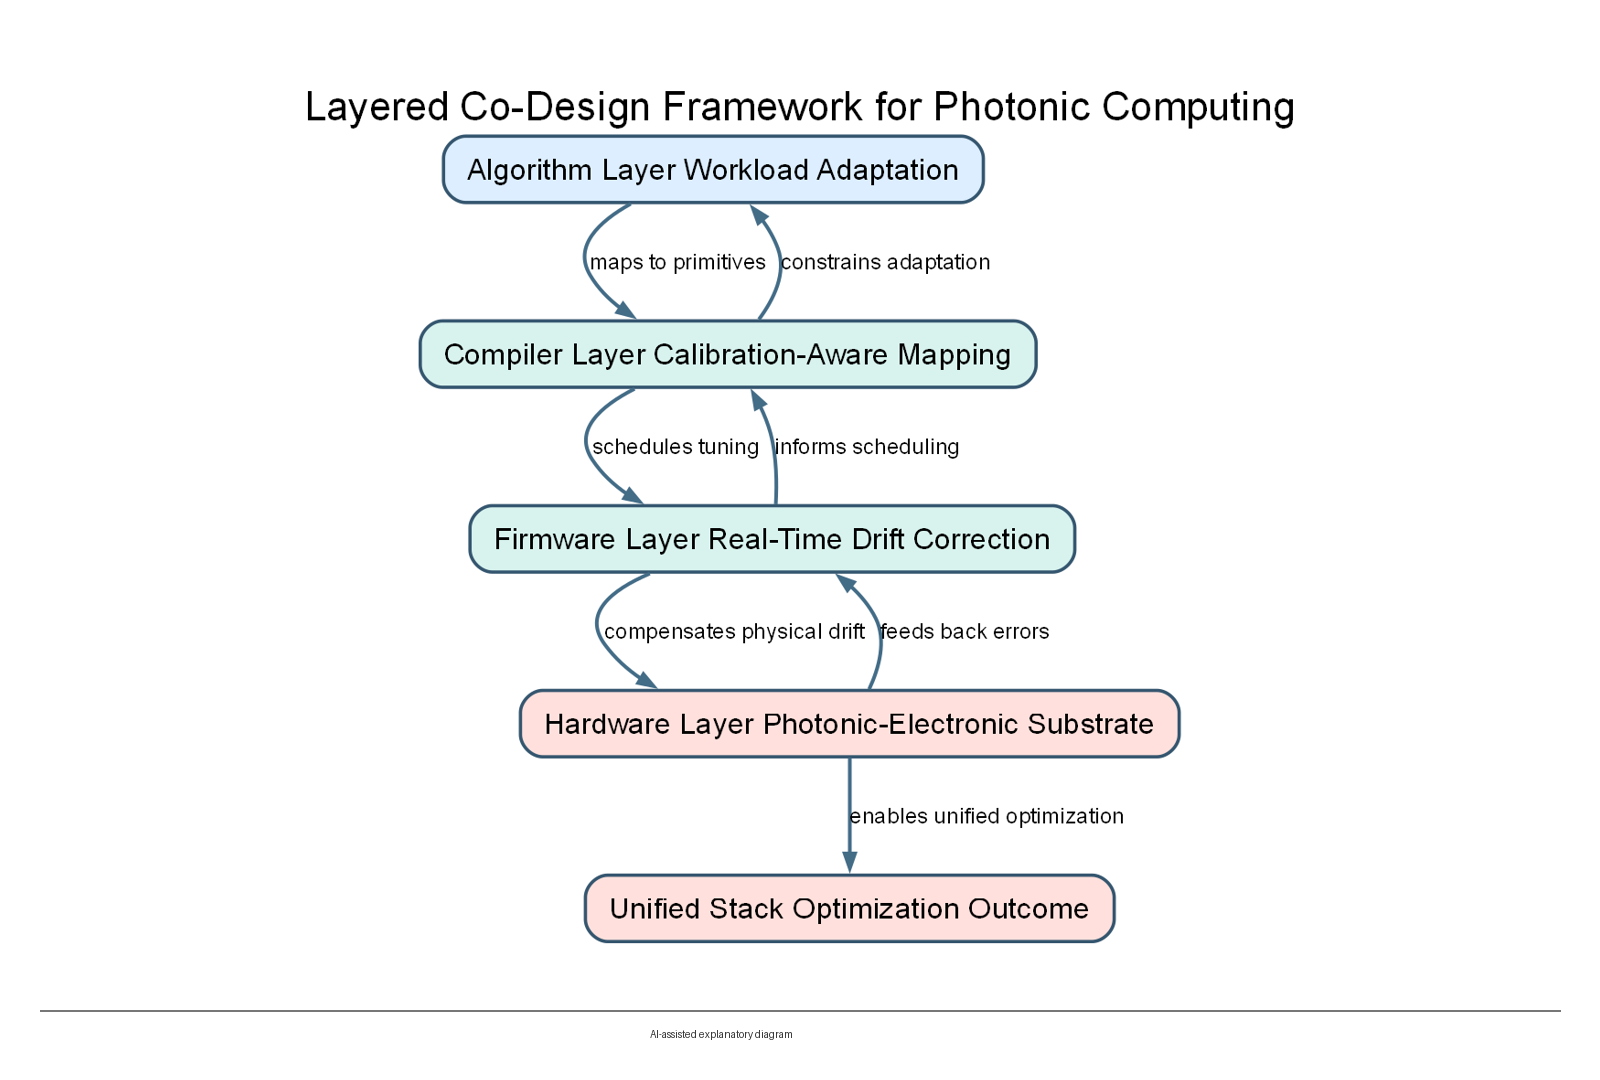
\includegraphics[width=0.9\linewidth,height=\textheight,keepaspectratio,alt={Layered Co-Design Framework for Photonic Computing. Co-design treats the entire stack as a unified optimization problem rather than optimizing components independently. AI-assisted explanatory diagram; not empirical evidence.}]{figures/02_FIG-GEN-004.png}
\caption{Layered Co-Design Framework for Photonic Computing. Co-design treats the entire stack as a unified optimization problem rather than optimizing components independently. AI-assisted explanatory diagram; not empirical evidence.}\label{fig:visual_02}
\end{figure}

Physics-informed neural networks (PINNs) represent a critical evolution in data-driven inverse design by embedding physical laws directly into the optimization loop to ensure realizability. Unlike traditional approaches that rely on post-hoc corrections, PINNs integrate governing partial differential equations directly into the loss function, effectively treating physical constraints as soft penalties during training. \citep{doi_10_1007_s10444_023_10065_9_12bf0652} \citep{s2_cc39d5405a933620426d86298fa8fe4cd51915c5_27626ee3} This mechanism allows deep convolutional mixture density networks to bypass conventional trial-and-error workflows, ensuring that algorithmic outputs for nanophotonic structures adhere to electromagnetic principles from the outset. To further accelerate this process, dynamic convolutional neural operators capture causal physical constraints, reducing the computational latency associated with traditional finite element methods. For instance, advanced architectures mitigate temporally accumulated errors in photonic device simulation by employing stage-dedicated prediction models and cross-stage hidden state propagation, aligning non-ideal input fields with ground-truth dynamics. While adjoint methods may offer higher accuracy in specific low-dimensional tasks, PINNs provide superior scalability because their computational cost depends on network architecture rather than mesh resolution, avoiding the intractable memory footprints of full discrete trajectory storage in high dimensions. By fusing artificial intelligence with physics-guided frameworks, these methodologies transform the co-design paradigm, enabling the rapid mapping of abstract functions to manufacturable device geometries without sacrificing physical fidelity. \citep{doi_10_48550_arxiv_2406_17810_813bd2a3} \citep{s2_037e66f37189104d61c0d000de0cee202b7eec9e_d15b8018} \citep{doi_10_48550_arxiv_2606_12337_68b62bfa}

Physics-informed architectures ensure adherence to governing equations, yet the transition from simulation to fabrication introduces two critical barriers: non-uniqueness and sensitivity to manufacturing variations. Inverse design in nanophotonics inherently faces a non-uniqueness problem where distinct meta-atom geometries yield identical optical properties, complicating the identification of a single optimal solution during co-design optimization. Deep learning approaches address this by leveraging unsupervised methods to automatically distinguish between different geometry groups, such as cross, split-ring, and h-shaped antennas, without explicit labeling, thereby stabilizing the search space. However, satisfying functional specifications alone does not guarantee experimental success if the resulting device is fragile against fabrication imperfections. To mitigate this, robust co-design methodologies incorporate strict foundry constraints, such as minimum length scales, directly into the optimization loop using techniques like design space reparameterization. \citep{doi_10_1021_acsphotonics_2c00313_0d7d39c3} By evaluating performance across eroded and dilated geometric variants within the loss function, these methods produce devices that maintain high efficiency despite width variations, effectively bridging the gap between theoretical performance and manufacturable reality. This robustness ensures that the unified optimization of hardware geometry and algorithmic structure remains viable when subjected to the physical tolerances of real-world foundries. \citep{doi_10_1515_nanoph_2019_0474_d2187501} \citep{doi_10_1021_acsphotonics_0c01202_d9ad1299} \citep{doi_10_1021_acsphotonics_2c00313_0d7d39c3}

Specific architectural paradigms now demonstrate how physical layers can directly implement algorithmic functions. Diffractive Optical Neural Networks (DONNs) represent a co-design approach where physical diffractive layers are jointly optimized with the target algorithmic function, enabling compact on-chip machine learning without iterative electronic feedback loops. This architecture has evolved from foundational free-space implementations to integrated on-chip configurations that enhance compatibility with photonic circuits while maintaining scalability in neuron count and ultra-high throughput. However, in scenarios requiring multi-wavelength parallel computation, operations are typically limited to a small number of widely separated wavelengths within a broad spectral band. Integrating diffractive elements with advanced wavelength-based modulation devices, such as photonic crystal microcavity arrays, offers a pathway to overcoming this limitation. These artificial bandgap materials enable precise manipulation of photon local density of states through periodic dielectric structures; by intentionally disrupting periodicity to create defect modes, they localize photons at specific frequencies to achieve optical signal control with wavelength precision. \citep{doi_10_1371_journal_pone_0341241_2b7bcccf} \citep{doi_10_1109_isset62871_2024_10779731_6ff2a9a8} This allows independent control of multi-wavelength optical signals through the design of defect structures, bypassing the wavelength-dependent phase modulation limitations inherent to conventional diffractive networks. Extending this concept, Physical Neural Networks (PNNs) enable co-design by allowing physical layers to implement controllable functions that are not mathematically isomorphic to conventional deep learning layers, thereby decoupling algorithmic structure from rigid hardware constraints. In PNNs, diverse physical systems---ranging from multimode mechanical oscillations to ultrafast optical second-harmonic generation---serve as hierarchical classifiers that inherently mitigate unique noise processes through their specific physical transformations. These architectures illustrate the chapter's central thesis: treating hardware geometry and algorithmic structure as a unified optimization problem allows photonic computing to bypass the limitations of simply substituting electronic components, though the practical deployment of such systems must still address the electronic control overheads detailed in the following section. \citep{doi_10_1002_nap2_70098_8d5f2f8a} \citep{doi_10_1038_s41586_021_04223_6_6158a5ea} \citep{doi_10_1515_nanoph_2025_0168_86a0f7aa}

Architectural paradigms like DONNs and PNNs enable compact on-chip learning, yet their physical realization faces a fundamental boundary condition: the electronic control overhead imposed by thermal crosstalk and fabrication variations. As detailed in Section 1, thermal crosstalk arises because the inevitable thermal conductance of chip materials allows heating from integrated thermo-optic phase shifters to spread, causing undesired interference that can lead to loss of confinement, reduced output power, or erroneous signal routing in dense circuits. \citep{doi_10_1109_access_2020_3013116_8fec1fb2} Although strategies such as three-dimensional trenches or doped silicon heaters placed close to waveguides aim to localize heating and improve efficiency, standard approaches often suffer from large footprints, high power consumption, or incompatibility with CMOS processes due to external heat sink requirements. Compounding this issue are fabrication-induced phase variations (FPVs), which introduce optical phase noise that degrades the accuracy of matrix-vector multiplication in coherent MZI based networks. Evidence indicates that optimizing nominal waveguide widths, particularly in etched ridge waveguides rather than strip waveguides, can significantly recover nominal accuracy under expected width and thickness variations. However, this tolerance is sensitive to the correlation length of variations; shorter correlation lengths cause fluctuations to change more rapidly within a region, imposing higher errors on region-based tolerant designs. Consequently, achieving scalability requires co-design approaches that treat these physical non-idealities as integral constraints during the algorithmic mapping and calibration process. \citep{doi_10_1109_access_2020_3013116_8fec1fb2} \citep{doi_10_1109_tnano_2022_3223915_d4da3e6b}

To mitigate electronic control overhead, advanced optimizers automate the mapping of abstract algorithmic objectives to physical device geometries. Reinforcement learning (RL) algorithms prove particularly effective for this inverse design in high-dimensional, non-convex parameter spaces where traditional heuristics often stagnate in local minima. By treating design as a sequence of states, actions, and rewards, methods like Deep Q-learning explore vast state-action spaces to discover optimal photonic crystal cavities that satisfy specific optical responses. \citep{doi_10_1515_nanoph_2022_0692_4b166807} Complementing this, systematic benchmarks reveal that machine learning optimizers, specifically Adam derivatives and Fromage, consistently outperform standard quasi-Newton methods like L-BFGS across varying system sizes, while meta-optimization can elevate simpler gradient methods to comparable performance levels. To further reduce computational burdens, scalable photonic neural networks employ surrogate scattering-matrix inverse design. That implementation models trainable optical stages as passive linear operators parameterized by unitary matrices and singular values, enforcing passivity and insertion-loss bounds directly within the optimization loop. \citep{s2_753a5d83a96e0194da93bcb6f20fa0bd356e37fa_c11e3796} By replacing expensive electromagnetic simulations with efficient matrix products during the exploratory phase, these surrogates enable rapid co-optimization of device geometry and system-level operators for tasks such as all-optical classification. Together, these automated frameworks bridge the gap between high-level functions and low-level hardware configurations, fulfilling the co-design imperative of unified optimization. \citep{doi_10_1515_nanoph_2022_0692_4b166807} \citep{doi_10_1063_5_0238444_48bf2cbe} \citep{s2_753a5d83a96e0194da93bcb6f20fa0bd356e37fa_c11e3796}

The ultimate realization of scalable photonic computing depends on heterogeneous integration platforms that physically unify optical substrates with electronic control planes, building upon the automated mapping strategies discussed previously. BEOL integration represents a critical advancement by combining thin-film lithium niobate (TFLN) with active silicon photonics on a single chip, thereby overcoming the latency and power overhead inherent in discrete packaging. The same strategy leverages the mature CMOS compatibility of silicon while incorporating TFLN's superior modulation efficiency and low loss, creating a tri-layer environment capable of supporting complex system-level functionalities like photonic computing. Complementing this hardware convergence, co-designed systems increasingly employ physics-informed neural networks (PINNs) to embed physical laws directly into optimization workflows. By bypassing conventional trial-and-error methods, these AI-driven frameworks address the high computational costs of traditional inverse design, effectively reducing the electronic control overhead required to map abstract algorithmic objectives to specific hardware configurations. Together, these monolithic integration techniques and physics-guided design methodologies define the trajectory toward fully integrated, cost-effective photonic transceivers and computing systems. \citep{s2_9b444e84d20ae6e3d62d2d4df30268b5a53baad2_40af2cc9} \citep{s2_037e66f37189104d61c0d000de0cee202b7eec9e_d15b8018}

\section{Photonic AI Acceleration within Scalable Photonic Computing Systems: Workload Mapping, Co-Design, and Performance Benchmarks}\label{photonic-ai-acceleration-within-scalable-photonic-computing-systems-workload-mapping-co-design-and-performance-benchmarks}

Photonic neural networks establish a distinct operational advantage for inference by leveraging the inherent physical properties of light to execute linear algebra naturally, building on the physical constraints of precision and noise established in prior sections. These systems utilize the superposition of complex optical waves and multi-cascade interferometry to perform transformations that are fundamentally compatible with deep neural network operations, effectively mapping mathematical requirements directly onto physical propagation. \citep{doi_10_1007_s11075_025_02218_2_e396aae0} \citep{doi_10_48550_arxiv_2510_03186_c4d4955e} To implement the necessary nonlinear activation functions without electronic conversion bottlenecks, architectures often exploit the inherent nonlinear behavior of optical resonators, although this design introduces sensitivity to environmental factors like temperature fluctuations and mechanical vibrations. Alternatively, interferometers excel in manipulating signal phase and amplitude for complex computations through inherent parallel processing, yet they require precise alignment and remain susceptible to phase variations. Currently, integrated matrix-vector multiplication engines primarily rely on Mach-Zehnder interferometer arrays or micro-ring resonator networks to realize these linear transformations. \citep{doi_10_1117_12_2690776_82e594d2} \citep{doi_10_54254_2753_8818_2026_33628_f99a21e9} While these integrated solutions offer compact structures compared to bulky free-space diffraction systems, they face significant hurdles in large-scale deployment, including the need for extremely precise phase control, complex feedback circuits, and limitations imposed by waveguide cross-talk and loss. This physical foundation delivers high-throughput capabilities for static tasks but simultaneously exposes the rigidity that complicates dynamic weight updates, setting the stage for examining the specific performance boundaries between efficient inference and challenging training workloads. \citep{doi_10_3390_nano14080697_c372a140} \citep{s2_b765388f3cc18d6e5a0507522822def0e3503ec6_fa09b483} \citep{doi_10_1088_1402_4896_ae8345_3b948559}

The exceptional energy efficiency of fixed linear transformations in photonic systems, enabled by the physical principle of superposition, diminishes sharply when transitioning from static inference to dynamic training. Integrated photonic tensor cores indeed demonstrate high throughput-per-watt for parallel convolutional processing where weights remain constant, yet training workloads introduce a fundamental mismatch by requiring frequent weight updates and gradient computations that rigid optical hardware cannot natively support. To bridge this gap, published studies have developed dual-neuron optical-artificial learning strategies, such as the DANTE framework, which hybridize the system by using optical neurons for forward propagation while relying on electronic artificial neurons to manage complex weight updates. The DANTE framework exemplifies this hybrid approach by employing dual-neuron optical-artificial learning, where optical neurons handle forward propagation while electronic artificial neurons manage complex weight updates during training. \citep{doi_10_1038_s41467_023_42984_y_7fc109e3} The proposed network becomes necessary because online in-situ training on purely photonic hardware faces severe latency challenges; for instance, compensating for system errors in high-dimensional tasks like MNIST classification can take prohibitively long due to environmental instabilities affecting optical paths. Consequently, while pure photonic replacement of electronic GPUs remains elusive for training, these hybrid control loops illustrate that realizing scalable optoelectronic neural networks demands a shift toward algorithm-hardware co-design, a topic explored in the following section. \citep{doi_10_1515_nanoph_2022_0423_38a2c3ec} \citep{doi_10_1038_s41467_023_42984_y_7fc109e3} \citep{doi_10_1038_s41467_022_35772_7_90150ade}

Algorithm-hardware co-design emerges as a critical strategy to overcome the rigidity of static photonic hardware identified in training loops, defined here as the joint optimization of neural network architectures and photonic device geometries to navigate physical constraints. \citep{doi_10_1109_dac63849_2025_11133307_892a6228} \citep{s2_c41720a8a362c412dc17bab4c3f329f2ac7c9818_1a5c96e4} The configuration directly addresses the failure of heuristic methods that oversimplify transfer matrices, which often yield unimplementable responses because they ignore the intricate wave interference and complex light-matter interactions governing the valid subspace of optical physics. Rigorous enforcement of these physical realities via partial differential equation (PDE) constraints is traditionally prohibitively expensive due to the computational cost of fullwave simulations, creating a non-convex optimization landscape that traps training in poor local optima. Deep learning-based inverse design methods resolve this bottleneck by serving as efficient surrogates or direct solvers that map desired optical responses to physical structures, such as metasurfaces or photonic crystals, without requiring exhaustive iterative simulations for every new target. By benchmarking models like tandem networks and generative adversarial networks, researchers can now prioritize not only accuracy but also the diversity and robustness of designs against fabrication variations, ensuring that proposed accelerators remain physically realizable. Consequently, co-design transforms the hardware-algorithm mismatch from a fundamental barrier into a manageable optimization problem, enabling photonic systems to better align with specific AI workload requirements while respecting the limits of nanofabrication. \citep{doi_10_48550_arxiv_2505_18377_a6fc9ec3} \citep{doi_10_1364_prj_415960_cf59d95b} \citep{doi_10_29026_oes_2022_210012_27973a69}

Advanced inverse design strategies now employ machine learning to bridge the gap between abstract device requirements and physical realization, building on the necessity for co-design established in the previous section. A primary approach involves dimensionality reduction techniques, which compress the complex design and response spaces of nanophotonic structures to reveal underlying physics while significantly lowering computational complexity; this enables an evolutionary design method where initial configurations are intelligently refined for robustness and lower power consumption. Complementing this, discriminative deep learning models accelerate optimization by bypassing repeated, computationally expensive electromagnetic simulations. For instance, bidirectional networks can learn the mapping between geometry and optical spectra, converging within hours to allow subsequent queries for potential nanostructures to be completed in milliseconds. To further embed physical rigor, physics-informed neural networks and differentiable simulators act as computational accelerators for metasurfaces and waveguides, utilizing compact wave priors to achieve simulation speeds orders of magnitude faster than traditional numerical solvers while reducing prediction errors. Finally, generative deep neural networks serve as efficient surrogate models for tunable devices like wavelength de-multiplexers; by exploring statistical structures to propose candidates, these workflows reserve costly full-wave evaluations only for the most promising designs, thereby balancing exploration speed with verification reliability. Collectively, these methods transform inverse design from a bottleneck into a scalable engine for realizing the high-performance photonic architectures discussed next. \citep{doi_10_1117_12_2595199_6f40f1c0} \citep{doi_10_1515_nanoph_2021_0660_2d91a441} \citep{doi_10_48550_arxiv_2209_10098_b3bedb78} \citep{doi_10_1109_access_2026_3697666_bd5258a6}

Recent demonstrations confirm that the inverse design strategies outlined previously yield functional, ultra-compact accelerators capable of high-performance inference on standard benchmarks. Recent work has demonstrated inverse-designed nanophotonic neural network accelerators that achieve ultra-compact optical computing capabilities. \citep{doi_10_1038_s41467_026_68648_1_26658a9c} In these architectures, input features are encoded onto coherent optical amplitudes which then undergo complex interference within a topology-optimized scattering region, effectively routing energy to specific output ports that represent class probabilities without electronic intermediate processing. For instance, inverse-designed nanophotonic neural networks have achieved 99.1\% numerical accuracy on the MedMNIST dataset, with optimized material topologies concentrating optical power at the correct output port while suppressing neighboring channels. Similarly, surrogate-assisted approaches have transferred target matrices to physical devices with minimal performance degradation, reaching 98.16\% test accuracy on all-optical classification tasks after only 20 optimization epochs. Beyond classification, deep neural network-based inverse design has automated the creation of integrated components like power splitters, achieving correlation coefficients greater than 0.995 across transmission ratios. These results validate the viability of algorithm-hardware co-design for static workloads, demonstrating that photonic systems can deliver compact, energy-efficient inference when the linear transformation is fixed, even as the challenge of dynamic reconfigurability for training remains addressed in subsequent scaling discussions. \citep{doi_10_1038_s41467_026_68648_1_26658a9c} \citep{s2_753a5d83a96e0194da93bcb6f20fa0bd356e37fa_c11e3796} \citep{s2_0482241c1bd933adb55a6674133d1688626bdab1_17e7627d}

Scaling inverse-designed accelerators to practical dimensions requires architectural innovations that overcome physical bottlenecks in integration and parallelism. One critical pathway is heterogeneous back-end-of-line (BEOL) integration, which combines thin-film lithium niobate (TFLN) with active silicon photonics on a single chip. \citep{s2_9b444e84d20ae6e3d62d2d4df30268b5a53baad2_40af2cc9} The resulting design leverages TFLN's superior modulation efficiency and low loss while retaining CMOS compatibility, creating a viable platform for the dense optical interconnects needed for high-throughput matrix operations. Alternatively, single-shot matrix-matrix processors attempt to bypass sequential limitations by using spatial-spectral hypermultiplexed parallel diffraction to perform matrix-vector multiplication in one step via wavelength-time interleaving. \citep{doi_10_1038_s41467_026_68452_x_bafa2de0} However, this method faces strict scaling boundaries due to the requirement for \(O(N^{2})\) comb lines and precise dispersion management, contrasting with architectures that suffer from fan-in losses or limited bit precision. A third strategy employs passive linear operators optimized through surrogate scattering-matrix inverse design, which encodes reduced-dimensionality feature vectors without requiring active weight updates during operation. By constraining singular values to enforce passivity, these networks enable scalable acceleration for fixed tasks like all-optical classification, though they inherently lack the dynamic reconfigurability of electronic counterparts. Together, these mechanisms illustrate that while hardware scalability is achievable through specialized integration and multiplexing, the trade-offs between component complexity, precision, and flexibility reinforce the chapter's thesis: realizing robust photonic AI demands co-design strategies that align algorithmic constraints with the specific physical capabilities of the underlying optical substrate. \citep{s2_9b444e84d20ae6e3d62d2d4df30268b5a53baad2_40af2cc9} \citep{doi_10_1038_s41467_026_68452_x_bafa2de0} \citep{s2_753a5d83a96e0194da93bcb6f20fa0bd356e37fa_c11e3796}

Architectural innovations like heterogeneous integration and single-shot processing address physical scaling, but the reliability of these systems depends on rigorous uncertainty quantification and efficient design workflows. Small-perturbation automatic differentiation (SPAD) offers a mechanism to handle input parameter uncertainties by exploiting separable derivative expansions, a approach that remains valid specifically when those uncertainties are small. This method separates probabilistic aspects from the core computational approach, allowing rapid recomputation for changes in probability distributions with linear complexity for uncorrelated variables. Complementing this, deep learning surrogates significantly reduce the computational costs associated with traditional electromagnetic simulations that typically require high-performance computing resources. Furthermore, physics-informed neural networks and mixture density networks enable robust inverse design by incorporating physical constraints and explicitly handling fabrication uncertainty distributions, thereby addressing the ill-posed nature of inverse scattering problems. These algorithmic advances mitigate some risks of hardware rigidity, yet they also highlight that without standardized system-level benchmarks, the true impact of these co-design strategies on end-to-end performance remains difficult to quantify. \citep{s2_964fe0d656467421d5df282abd0e0a2aca877e7e_399e029e} \citep{doi_10_1109_sbfotoniopc62248_2024_10813471_692f0088} \citep{s2_037e66f37189104d61c0d000de0cee202b7eec9e_d15b8018}

ODNN research faces critical open questions regarding the path to functional, system-level photonic AI accelerators, building on acknowledged limitations in uncertainty quantification and the absence of standardized benchmarks. First, it remains an open question whether the tight integration of electronic control and memory subsystems with photonic computing engines is a strict architectural requirement for viability, as the available material lacks specific benchmark data comparing such hybrid systems against established electronic GPUs or TPUs for standard machine learning workloads. Second, current research efforts may disproportionately focus on component-level metrics, such as modulator speed and waveguide loss, rather than providing end-to-end system-level benchmarks normalized to established standards like FLOPS per Watt for specific AI model architectures; the evidence set does not establish the extent of this disparity. Finally, while precision limitations are known, it is not yet established by the available material whether specific algorithm-hardware co-design strategies, such as quantization-aware training or sparsity exploitation, are strictly necessary to mitigate these hardware constraints during deep learning execution. These gaps highlight that realizing the chapter's thesis---that co-design is the critical enabler---requires a shift from isolated component demonstrations to rigorous, holistic system validation.

\section{Optical Interconnect Fabrics for Distributed Scalable Photonic Computing Systems}\label{optical-interconnect-fabrics-for-distributed-scalable-photonic-computing-systems}

Optical signal processing represents a fundamental shift from electrical domain constraints, offering wide-bandwidth capabilities, cost-effectiveness, and superior power efficiency while providing strong immunity to electromagnetic interference. As global demands for high data rates escalate to support applications like autonomous driving and the Internet of Things, existing electronic solutions face critical limitations in power consumption and bandwidth operation, necessitating a transition to programmable processors based on integrated silicon photonics. Silicon photonics has emerged as a promising transmission medium for chip-to-chip communication specifically because it delivers lower channel losses, reduced crosstalk, and minimized dispersion compared to electrical signaling through copper lines. This viability is demonstrated by architectures such as OptoLink, which exploits Wavelength and Space Division Multiplexing to achieve ultra-high throughput; specifically, such designs have reached 1.6 TB/s of bandwidth across 128 optical channels, representing a 300-fold latency reduction compared with conventional electronic networks. OptoLink addresses memory bandwidth bottlenecks in FHE accelerators by employing Wavelength and Space Division Multiplexing at the chiplet scale. This photonic interconnect architecture achieves up to 1.6 TB/s of bandwidth across 128 optical channels, effectively overcoming the inefficient memory transfers and off-chip communication overheads that constrain recent hardware designs. \citep{doi_10_1145_3806395_315ab915} By alleviating memory transfer delays by orders of magnitude, these photonic interconnects directly address the bottlenecks that constrain modern computing fabrics, establishing the essential performance foundation upon which advanced inverse design methodologies must build to overcome remaining integration challenges. \citep{doi_10_1109_access_2020_3013116_8fec1fb2} \citep{doi_10_1145_3806395_315ab915} \citep{doi_10_1007_s11082_024_08009_8_0f7f241e}

Scalable photonic computing relies on nanophotonic inverse design, a computational approach that determines optimal device geometries for target optical responses rather than relying on human intuition, to overcome the bandwidth and energy constraints of electrical links established previously. \citep{doi_10_1002_lpor_202503115_6bf85dd2} \citep{doi_10_1039_d4nr03081h_5c44e89e} Unlike traditional trial-and-error modeling which yields only incremental advancements, inverse design techniques explore the full parameter space to implement non-intuitive optical structures critical for compact interconnect components, ranging from beam splitters to metalenses. This framework shift is accelerated by deep learning frameworks, where neural networks are trained on large datasets of electromagnetic simulations to intelligently learn the nonlinear relationships governing light propagation, effectively approximating Maxwell's equations without explicit programming. Once trained, these models facilitate the rapid optimization of device geometries to meet specific spectral responses, solving design requests almost instantaneously compared to the cycles required by conventional gradient-based or evolutionary algorithms. However, this data-driven efficiency comes with significant boundaries; generating the necessary training datasets requires extensive upfront computational resources and time-consuming simulations, creating a barrier to scaling these methods for highly complex devices. Furthermore, the performance of deep learning-designed devices is inherently limited by the quality and scope of their training data, often necessitating additional optimization processes to exceed existing benchmarks. Despite these challenges, the fusion of optimization schemes with deep learning predictors offers a viable path toward miniaturizing optical systems, directly supporting the chapter's thesis that co-optimizing photonic substrates with advanced design methodologies is essential for realizing high-density optical interconnect fabrics. \citep{doi_10_1515_nanoph_2021_0660_2d91a441} \citep{doi_10_1515_nanoph_2024_0536_4b6631ba} \citep{doi_10_1515_nanoph_2018_0183_d85e9193} \citep{doi_10_1515_nanoph_2019_0474_d2187501}

Specific deep learning architectures now enable the rapid optimization of nanophotonic components essential for dense optical interconnect fabrics, building on the foundational concept of inverse design. Generative deep neural networks and adversarial autoencoders serve as powerful tools to map desired optical responses directly to device geometries, bypassing the time-consuming iterative simulations required by conventional methods. For instance, conditional generative adversarial networks (CGANs) have been developed to generate lithographic masks for meta-atoms with predefined transmission and reflection properties, facilitating the creation of complex metasurfaces and photonic crystal waveguides. Conditional generative adversarial networks (CGANs) have been utilized for the inverse design of metamaterials and photonic crystals. Specifically, these neural networks generate lithographic masks for meta-atoms with desired transmission and reflection properties, enabling the creation of complex structures such as metasurfaces and nonlinear photonic-crystal waveguides. \citep{doi_10_1109_metamaterials62190_2024_10703328_b89eaef7} Similarly, these data-driven approaches are increasingly applied to design integrated silicon nanophotonic gratings, which are critical for vertical light coupling in CMOS-compatible systems. Beyond simple accuracy, advanced methods like variational autoencoders (VAEs) and tandem networks are being benchmarked for their ability to produce diverse design candidates and ensure robustness against fabrication variations, addressing the practical need for structures with smooth shapes and low aspect ratios. Furthermore, representation learning techniques mitigate computational bottlenecks by creating reusable, physics-agnostic manifolds of device geometries; this allows global optimization schemes to explore design spaces more efficiently without the prohibitive cost of full-wave electromagnetic simulations at every step. While these architectures significantly accelerate the design of spectral tuning and phase control elements, their reliance on training data and potential sensitivity to fabrication tolerances highlight the need for further integration with physical constraints, a challenge addressed in the following section. \citep{doi_10_1109_metamaterials62190_2024_10703328_b89eaef7} \citep{doi_10_1109_cleo_europe_eqec52157_2021_9542763_c5b6331c} \citep{doi_10_29026_oes_2022_210012_27973a69} \citep{doi_10_1002_adom_202502062_d73a85e1}

Deep learning architectures accelerate device optimization, yet purely data-driven neural networks often struggle to generalize beyond their specific training distributions, limiting their robustness in novel interconnect configurations. To overcome this, hybrid algorithms have emerged that combine the global search capabilities of neural networks with conventional optimization methods for local refinement. A more integrated solution involves Physics-Informed Neural Networks (PINNs), which embed physical laws directly into the optimization workflow rather than relying solely on data patterns. \citep{doi_10_1038_s41467_025_64624_3_42144da5} \citep{doi_10_3390_s25196242_b7203a7f} By incorporating differentiable physical simulators or adjoint-based methods into the training pipeline, these models enable parameter-efficient optimization of complex nanophotonic structures. For instance, physics-informed reinforcement learning has demonstrated significantly higher sample efficiency in designing freeform metasurfaces compared to standard approaches, while other frameworks achieve faster simulation speeds with reduced prediction errors across unseen settings. This shift toward physics-constrained design ensures that scalable photonic computing fabrics maintain performance fidelity even as device geometries become increasingly intricate. \citep{doi_10_1021_acsphotonics_2c00968_06a2e96b} \citep{s2_037e66f37189104d61c0d000de0cee202b7eec9e_d15b8018} \citep{doi_10_1515_nanoph_2023_0852_cb27a26f} \citep{doi_10_48550_arxiv_2209_10098_b3bedb78}

Translating physics-informed designs into mass-producible components necessitates adapting inverse design methodologies to strict foundry fabrication constraints. To address this, manufacturability is enforced by subjecting the optimization process to hard limits such as minimum length scales and brush size restrictions, transforming the design task into a combinatorial problem that is approximately solved via stochastic gradient optimization with conditional generators. This ensures that generated photonic components remain feasible for large-scale deployment within existing semiconductor processes. Furthermore, deep reinforcement learning empowers automated optimization by treating device tuning as a sequential decision process, allowing agents to learn policies that satisfy tight resonance wavelength tolerances essential for high-quality lasing and telecommunications. Deep reinforcement learning has been applied to the automated inverse design and optimization of photonic crystals, specifically for creating nanoscale laser cavities. \citep{doi_10_1515_nanoph_2022_0692_4b166807} Complementing these constraint-aware methods, deep learning models serve as efficient surrogates for forward prediction, learning the mapping between structural parameters and optical responses to bypass the computational expense of traditional electromagnetic simulations. Unlike target-specific optimization methods that must restart for every new design goal, these surrogate models generalize across problems, predicting optimal structures within milliseconds and significantly accelerating the path from simulation to fabrication. Together, these advances bridge the gap between theoretical performance and practical manufacturability, a prerequisite for the scalable optical interconnect fabrics central to this chapter's thesis. \citep{doi_10_1021_acsphotonics_2c00313_0d7d39c3} \citep{doi_10_1515_nanoph_2022_0692_4b166807} \citep{doi_10_29026_oes_2022_210012_27973a69} \citep{doi_10_1109_jphot_2022_3182050_3cfb78ba}

Realizing scalable photonic fabrics ultimately depends on advanced material platforms that enable dense, active integration beyond the limits of pure silicon. BEOL integration addresses this by combining thin-film lithium niobate (TFLN) with active silicon photonics on a single substrate, a process that overcomes traditional die-to-wafer bonding challenges to co-package high-performance transceivers and computing accelerators. Heterogeneous back-end-of-line integration enables the combination of thin-film lithium niobate with active silicon photonics on a single substrate to achieve single-chip optical transceivers. \citep{s2_9b444e84d20ae6e3d62d2d4df30268b5a53baad2_40af2cc9} Unlike passive silicon circuits, this hybrid platform leverages TFLN's intrinsically low loss and superior modulation efficiency while retaining CMOS compatibility for mature silicon photonic components. The active control required for such dynamic routing stems from lithium niobate's unique ferroelectric properties, where `electric-field poling' allows the local inversion of spontaneous polarization at room temperature to engineer electro-optic coefficients without obsolete high-temperature diffusion processes. \citep{s2_a1b7de5981aa9a6aa9f9bd0c4422d9b023fc454f_bec494c5} \citep{doi_10_1117_12_2654937_d0b4bc2b} Complementing these volumetric materials, on-chip dielectric metasurfaces provide a CMOS-compatible mechanism to control the degrees of freedom of the light field, serving as arbitrary wavefront shapers for compact, broadband operations like convolution. Although current modulators and detectors have not yet reached their ultimate performance limits, this tri-layer integration of silicon, TFLN, and silicon nitride establishes a clear path toward complex system-level functionalities, directly addressing the memory bandwidth bottlenecks that constrain emerging applications like fully homomorphic encryption. \citep{s2_9b444e84d20ae6e3d62d2d4df30268b5a53baad2_40af2cc9} \citep{doi_10_1126_science_abj4396_40f36a09} \citep{doi_10_1515_nanoph_2022_0294_1bd118d5} \citep{doi_10_1145_3806395_315ab915}

Optical interconnects now address critical bottlenecks in secure and artificial intelligence computing domains, building on the heterogeneous integration capabilities described previously. In Fully Homomorphic Encryption (FHE), which enables computation directly on encrypted data for privacy-sensitive applications like healthcare, performance is often stifled by memory bandwidth limitations during operations such as CKKS bootstrapping. The OptoLink architecture alleviates this constraint by employing Wavelength and Space Division Multiplexing at the chiplet scale to deliver up to 1.6 TB/s of bandwidth across 128 optical channels. The optical architecture reduces latency by a factor of 300 compared to conventional electronic networks and improves bootstrapping throughput by up to 11 times, effectively enabling practical large-scale FHE acceleration. Parallel advancements in AI are realized through Diffractive Optical Neural Networks (DONNs), which utilize compact, passive on-chip structures to achieve ultra-high throughput and low-power operation for machine learning tasks. Complementary integrated photonic tensor cores further support these efforts by facilitating parallel convolutional processing and high-bandwidth data movement within tiled optical architectures. Together, these applications demonstrate that optical interconnects provide the necessary bandwidth density to overcome the scalability limits of electrical links, though realizing their full potential requires addressing the system-level thermal and co-design challenges discussed next. \citep{doi_10_1145_3806395_315ab915} \citep{doi_10_1002_nap2_70098_8d5f2f8a} \citep{doi_10_1515_nanoph_2022_0423_38a2c3ec}

Optical interconnects effectively resolve bandwidth bottlenecks in applications such as Fully Homomorphic Encryption, yet their dense integration introduces a critical physical limitation: thermal crosstalk. In integrated thermo-optic attenuators and phase shifters, the inevitable thermal conductance of chip materials causes heat from one component to diffuse into neighbors, creating undesired power fluctuations that restrict working capabilities and can lead to erroneous signal routing. Although strategies such as three-dimensional trenches or doped silicon heaters have been proposed to localize heating effects, existing designs often suffer from large footprints, high power consumption, or reliance on external heat sinks incompatible with standard CMOS processes. This device-level instability necessitates a broader co-optimization approach where inverse design is performed in isolation and is tightly coupled with system-level architectural constraints. As photonic neural networks scale, the accumulation of losses, dispersion, and noise across numerous optical modules requires hardware resources and software tools to jointly manage these thermal and loss bottlenecks. Consequently, realizing the full potential of scalable photonic computing demands that device fabrication and system architecture be co-designed to mitigate the physical interference that threatens the reliability of high-density optical fabrics. \citep{doi_10_1109_access_2020_3013116_8fec1fb2} \citep{doi_10_1145_3806395_315ab915} \citep{doi_10_3390_nano14080697_c372a140}

The preceding discussion highlighted thermal crosstalk and architectural co-design as immediate hurdles, yet two fundamental questions remain unresolved regarding the ultimate scalability of optical interconnect fabrics. First, although specific implementations like OptoLink demonstrate that photonic chiplet architectures can achieve 1.6 TB/s bandwidth and reduce latency by 300 times compared to electronic networks for Fully Homomorphic Encryption workloads, the available material does not definitively establish whether these gains translate into consistent orders-of-magnitude improvements in energy-per-bit and bandwidth-density across the broader spectrum of chip-to-chip and board-to-board scaling scenarios. Second, a critical gap persists in design methodology: current machine learning approaches appear heavily skewed toward component-level optimization rather than the holistic system-level co-design required to integrate interconnect fabrics directly with computing accelerators. While OptoLink successfully leverages Wavelength and Space Division Multiplexing to improve bootstrapping throughput by up to 11 times on specific platforms, it remains an open question whether existing inverse design frameworks can evolve from optimizing isolated devices to managing the complex trade-offs of distributed photonic computing systems. Resolving these uncertainties is essential to transition from promising point solutions to the mature, deployable technology envisioned by this chapter's thesis. \citep{doi_10_1145_3806395_315ab915}

\section{State of Scalable Photonic Computing: Synthesis, Benchmarking Gaps, and Trajectory Assessment}\label{state-of-scalable-photonic-computing-synthesis-benchmarking-gaps-and-trajectory-assessment}

Scalable photonic computing has undergone a fundamental paradigm shift from intuition-based design to data-driven inverse design, a methodological evolution essential for overcoming the geometric complexity limits of traditional approaches. Inverse design reverses the conventional simulation workflow by using optimization algorithms and artificial intelligence to determine device geometries directly from desired optical responses, thereby enabling non-intuitive structures that human heuristics often miss. \citep{doi_10_1117_12_3066105_d6297c38} \citep{doi_10_48550_arxiv_2506_18627_e2696034} This transition is powered by deep learning architectures, where discriminative models learn complex mappings between physical parameters and optical spectra to bypass repeated, computationally expensive full-wave electromagnetic simulations. For instance, bidirectional neural networks have demonstrated the ability to converge training within hours and subsequently generate valid nanophotonic layouts, such as split-ring resonators, in milliseconds. While generative models further expand this capability by sampling diverse optimal designs from a learned latent space, the approach faces boundaries; specifically, the initial training phase demands extensive labeled datasets derived from time-consuming simulations, and the resulting devices are constrained to perform within the bounds of their training distribution. Despite these computational overheads, this AI-driven foundation is critical for producing the optimized components required for system integration, setting the stage for the rapid simulation architectures discussed next to scale these designs further. \citep{doi_10_1515_nanoph_2021_0660_2d91a441} \citep{doi_10_1515_nanoph_2024_0536_4b6631ba}

Neural operators have emerged as a critical architecture for accelerating photonic simulation by learning mappings between function spaces rather than fixed input-output pairs, building on the shift toward data-driven inverse design established in prior sections. Unlike traditional surrogate models that regress high-dimensional vectors, frameworks such as DeepONets approximate nonlinear operators capable of accepting function-valued inputs like boundary conditions or source terms, allowing them to evaluate new scenarios at negligible cost while remaining differentiable for gradient-based optimization. \citep{doi_10_48550_arxiv_2406_05072_c02ad5f4} \citep{doi_10_1122_8_0000908_e28c4124} To further address the computational latency of traditional finite-difference time-domain solvers, recent advances introduce physics-inspired dynamic convolutional architectures that respect space-time causality constraints inherent in Maxwell's equations. These models mitigate the distribution shifts and accumulated roll-out errors typical of autoregressive predictions by employing stage-dedicated submodels and cross-stage hidden state propagation, ensuring that light field predictions align with ground-truth dynamics without violating physical locality. By replacing static matrix multiplications with mechanisms that capture permittivity-dependent wave propagation, these differentiable simulators significantly reduce the overhead associated with large-scale design tasks, directly addressing the computational bottlenecks that currently impede the fair benchmarking and scalable deployment of photonic systems. \citep{doi_10_48550_arxiv_2601_00199_c689b34d} \citep{doi_10_48550_arxiv_2406_17810_813bd2a3}

Embedding constraints directly into the learning process is required to ensure that generated geometries remain physically valid and manufacturable, even as neural operators and differentiable simulators accelerate the design loop. Physics-Informed Neural Networks (PINNs) address this by incorporating governing physical equations directly into the training objective via automatic differentiation, providing hard constraints that improve the physical consistency and reliability of inverse-designed photonic components compared to purely data-driven black-box models. \citep{doi_10_48550_arxiv_2606_12337_68b62bfa} \citep{doi_10_48550_arxiv_2603_09359_098af542} This fusion of artificial intelligence with physics-guided frameworks has opened transformative avenues for advancing the design and optimization of electromagnetic and nanophotonic systems, enabling robust tools to tackle longstanding challenges in light scattering engineering and meta-optics. To bridge the gap between theoretical performance and practical deployment, these methods are increasingly constrained by strict foundry fabrication limits, such as minimum length scales, which transform the design task into a combinatorial optimization problem solved through unconstrained stochastic gradient approaches. By utilizing conditional generators for feasible designs and straight-through estimators for backpropagation, inverse design methods can generate photonic device geometries that are both high-performance and manufacturable, directly addressing a critical barrier to scalable integration. However, the efficacy of these hard-constrained architectures depends on resolving multi-causal failure modes, including spectral bias and optimization imbalance, which can otherwise lead to loss-weight collapse even when physics-informed residuals appear minimized. \citep{s2_cc39d5405a933620426d86298fa8fe4cd51915c5_27626ee3} \citep{s2_037e66f37189104d61c0d000de0cee202b7eec9e_d15b8018} \citep{doi_10_1021_acsphotonics_2c00313_0d7d39c3}

Physics-informed constraints ensure manufacturability, yet underlying inverse design methodologies face profound computational hurdles rooted in high-dimensional, non-convex parameter spaces that often defy human intuition. Automated optimization frameworks are essential here, yet they encounter distinct efficiency limits: global stochastic methods suffer from the curse of dimensionality as sampling requirements grow exponentially, while gradient-based schemes risk converging to local optima within oscillatory objective landscapes. Compounding these algorithmic challenges, deep learning-based models introduce significant overhead through sensitivity to hyperparameter tuning and a lack of systematic evaluation regarding robustness against fabrication variations. Furthermore, current physics-informed machine learning approaches exacerbate this burden via bi-level and stochastic optimization requirements, which increase training complexity and currently limit immediate scalability for large-scale systems. A distinct challenge arises in purely generative approaches, which treat inverse design as a direct mapping problem learned through deep generative models or fine-tuned language models. Despite their appeal, such models face a persistent Constraint Rigor Gap, characterized by a difficulty in strictly enforcing hard physical or chemical constraints that are fundamental in scientific domains. Current generative frameworks typically handle these via soft penalties or regularization in their loss functions, leading to only partial constraint satisfaction and feasibility rates as low as 60-80\% in reported studies. These computational bottlenecks underscore that while component fidelity is achievable, the path to scalable deployment remains obstructed by optimization inefficiencies rather than fundamental physical limits. \citep{doi_10_48550_arxiv_2602_18148_e9c0a72b} \citep{doi_10_29026_oes_2022_210012_27973a69} \citep{doi_10_55041_ijsrem43509_b9a7bd5e} \citep{doi_10_48550_arxiv_2511_00070_bf8eda11}

Having addressed the computational overhead of inverse design, these methodologies now enable tangible hardware realizations through on-chip dielectric metasurfaces and heterogeneous integration. On-chip dielectric metasurfaces have emerged as a key technology for scalable photonic computing because they offer a unique scheme to control the degrees of freedom of the on-chip light field while remaining compatible with standard CMOS fabrication processes. This compatibility allows low-loss, broadband silicon photonic metasurfaces to serve as analog photonic accelerators capable of performing fundamental operations like convolution. Parallel to this, heterogeneous back-end-of-line (BEOL) integration platforms have successfully combined thin-film lithium niobate (TFLN) with active silicon photonics, overcoming critical challenges in die-to-wafer bonding and multilayer integration. Unlike previous efforts limited to passive circuits, that implementation integrates high-speed germanium photodetectors with high-performance TFLN modulators on a single chip, leveraging mature silicon photonics design kits to facilitate complex system-level functionalities. To ensure these physical structures are optimally realized, surrogate-based inverse design workflows decouple label fitting, fabrication-aware parameterization, and electromagnetic scattering into distinct stages. By first optimizing an optical block directly in matrix space and subsequently transferring the operator to a fabrication-aware device via an adjoint problem, this method mitigates the nonconvexity inherent in single-loop joint optimization and significantly reduces the computational cost per epoch. Together, these advances in metasurface control, heterogeneous material integration, and decoupled design workflows bridge the gap between abstract algorithmic requirements and manufacturable photonic systems, setting the stage for evaluating their performance in complete optical neural network architectures. \citep{doi_10_1515_nanoph_2022_0294_1bd118d5} \citep{s2_9b444e84d20ae6e3d62d2d4df30268b5a53baad2_40af2cc9} \citep{s2_753a5d83a96e0194da93bcb6f20fa0bd356e37fa_c11e3796}

Integrated diffractive photonic computing units now demonstrate viability as accelerators for specific artificial intelligence workloads, particularly all-optical graph representation learning. Unlike traditional electronic processors that struggle with the sequential demands of large-scale deep neural models, these photonic substrates leverage high parallelism and lightspeed signal processing to handle complex graph-structured data encoding relationships between entities. Diffractive optical neural networks (DONNs) represent a key architecture in this shift, utilizing passive low-power operation and scalable neuron counts to achieve ultrahigh throughput for inference tasks. However, while free-space and on-chip implementations offer distinct pathways toward intelligent computing, practical deployment faces significant hurdles including complex optical configurations, critical alignment requirements, and the lack of efficient optical nonlinear activation. To address these integration challenges, hybrid approaches such as only-train-electrical-to-optical-conversion systems have emerged, shifting adaptive training and nonlinear functions to the electronic domain while maintaining optical readout to avoid speed-limiting conversions. Although these simplified opto-electronic designs reduce calibration needs and enable reconfiguration without moving physical components, ODNN research remains constrained by fabrication tolerances and the absence of standardized benchmarks, setting the stage for a deeper examination of the evaluation gaps hindering fair comparison against electronic alternatives. \citep{doi_10_1126_sciadv_abn7630_4399f2ff} \citep{doi_10_1002_nap2_70098_8d5f2f8a} \citep{doi_10_1364_oe_462370_1269b480}

System-level demonstrations like OptoLink illustrate the transformative potential of photonic interconnects, achieving up to 1.6 TB/s bandwidth and a 300-fold latency reduction compared to electronic networks, yet these isolated successes underscore a critical fragmentation in evaluation methodologies. It remains an open question whether ODNN research currently lacks standardized benchmarking protocols that simultaneously account for energy efficiency and computational fidelity across diverse photonic modalities, which would impede fair comparison with electronic alternatives. Standardized benchmarking requires the consistent definition of operational parameters, such as specific wavelength ranges (e.g., 900 to 1100 nm) and deflection angles, to enable direct performance comparisons between different inverse design strategies. Without such consensus, reported metrics remain context-dependent, making it difficult to distinguish fundamental architectural advantages from optimization artifacts. Consequently, while specific applications like encrypted machine learning show promise, ODNN research currently lacks the standardized framework necessary to rigorously establish whether scalable photonic computing consistently outperforms electronic systems across broader workloads. \citep{doi_10_1145_3806395_315ab915} \citep{doi_10_1515_nanoph_2023_0852_cb27a26f} \citep{s2_9b444e84d20ae6e3d62d2d4df30268b5a53baad2_40af2cc9}

Addressing the identified benchmarking void, the trajectory of scalable photonic computing now suggests a distinct bifurcation in adoption pathways. While general-purpose photonic AI accelerators remain niche pending the resolution of standardized evaluation protocols, optical interconnects are poised for earlier widespread deployment in data centers due to their mature CMOS compatibility and immediate ability to address specific bandwidth bottlenecks. This divergence is exemplified by architectures like OptoLink, which leverages Wavelength and Space Division Multiplexing to deliver ultra-high throughput at the chiplet scale, achieving up to 1.6 TB/s of bandwidth and a 300-fold latency reduction compared to conventional electronic networks. Such system-level co-design, where artificial intelligence drives both device optimization and hardware implementation, has fundamentally shifted ODNN research from component-centric efforts to software-defined nanophotonic infrastructures that decouple hardware from end-user constraints. However, while these interconnects demonstrate clear advantages in alleviating memory transfer delays for workloads like Fully Homomorphic Encryption, it remains an open question whether the current lack of unified metrics for energy-per-operation and latency under realistic conditions will hinder the broader scaling of photonic AI accelerators relative to their electronic counterparts. \citep{doi_10_1145_3806395_315ab915} \citep{doi_10_1016_j_pquantelec_2023_100469_e4974ca6}

\section{Conclusion}\label{conclusion}

The evolution of scalable photonic computing, as synthesized from the preceding analysis of device physics, architectural primitives, and system-level integration, leads to a definitive conclusion: ODNN research has matured beyond the search for a singular ``silver bullet'' material or device. Instead, the path to practical deployment is defined by a strategic convergence of heterogeneous material platforms and rigorous electronic-photonic co-design. The central question of whether photonic systems can scale to meet the demands of next-generation computing is answered affirmatively, but with critical caveats regarding their operational domain. Photonic computing does not appear poised to universally replace electronic processors for general-purpose logic or high-precision training. Rather, its viability is established within a specialized envelope characterized by high-throughput, low-precision inference and ultra-high-bandwidth data movement, where the inherent parallelism and energy efficiency of light offer distinct advantages over charge-based electronics.

This conclusion rests on the fundamental trade-offs elucidated throughout the review. The dichotomy between silicon photonics, with its CMOS compatibility but weak electro-optic response, and thin-film lithium niobate, offering superior modulation efficiency at the cost of integration density, necessitates hybrid integration strategies. The body of evidence suggests that no single material platform currently satisfies all requirements for scale, speed, and energy efficiency simultaneously. Consequently, heterogeneous back-end-of-line integration emerges as a critical enabler, allowing disparate materials to be combined on a single substrate to leverage their respective strengths. However, this physical convergence is insufficient without addressing the systemic bottlenecks that arise at scale. The review identifies thermal crosstalk, cascaded insertion loss, and fabrication-induced variations as compounding barriers that degrade signal fidelity in dense arrays. These physical limitations are not merely engineering hurdles to be overcome by better fabrication; they represent fundamental boundary conditions that constrain the achievable circuit depth and control complexity.

Furthermore, the absence of native nonlinearity in passive photonic media imposes a structural limit on algorithmic applicability. While photonic matrix multiplication engines excel at linear algebra operations, the reliance on hybrid electronic mechanisms for activation functions and weight updates introduces latency and energy overheads that can erode theoretical performance gains. This reality reinforces the finding that purely photonic solutions are currently ill-suited for dynamic training workloads requiring frequent gradient computations. Instead, the most promising applications lie in static or slowly varying inference tasks and optical interconnect fabrics, where the rigidity of optical hardware aligns with the computational requirements. The success of architectures like OptoLink in alleviating memory bandwidth bottlenecks for Fully Homomorphic Encryption demonstrates that optical interconnects represent the most immediately deployable application of this technology, offering orders-of-magnitude improvements in bandwidth density compared to electrical links.

Looking forward, the trajectory of scalable photonic computing depends less on further component miniaturization and more on the adoption of holistic co-design methodologies. The traditional approach of optimizing devices in isolation is increasingly inadequate for navigating the complex, non-convex design spaces of wafer-scale systems. The integration of physics-informed machine learning and inverse design tools offers a pathway to automate the mapping of abstract algorithmic objectives to manufacturable device geometries, effectively treating hardware constraints as integral parts of the optimization loop. Yet, the realization of this potential is currently hindered by a fragmentation in evaluation methodologies. The lack of standardized benchmarks for energy-per-operation and computational fidelity across diverse photonic modalities impedes fair comparison with electronic alternatives and slows community convergence on best practices.

In summary, scalable photonic computing stands at an inflection point. The foundational physics and architectural primitives are well-understood, and the potential for transformative impact in specific domains is clear. However, bridging the gap between laboratory demonstrations and robust, system-level deployment requires a paradigm shift. Future progress will likely be driven not by isolated breakthroughs in device performance, but by the synergistic integration of advanced material platforms, intelligent design algorithms, and rigorous system-level validation. By embracing these co-design strategies and addressing the meta-challenges of benchmarking and standardization, ODNN research can transition from promising point solutions to the mature, deployable infrastructure envisioned for the post-Moore's law era.
